\chapter{\sc Two--Phase Stokes Flow}\label{ch:stokes}

This chapter is extensively based on a paper we wrote, see \cite{stokesfitted}.

\section{Mathematical model}\label{sec:stokes_model}
We consider two-phase Stokes flow in a given domain $\Omega\subset\R^d$, where
$d=2$ or $d=3$. As already described in \S\ref{sec:free_boundary_flows},
the domain $\Omega$ contains two different immiscible, incompressible, viscous
fluids (liquid-liquid or liquid-gas) which for all $t\in[0,T]$ occupy time
dependent regions $\Omega_+(t)$ and
$\Omega_-(t):=\Omega\setminus\overline{\Omega}_+(t)$ and which are separated by
an interface $(\Gamma(t))_{t\in[0,T]}$, $\Gamma(t)\subset\Omega$. In this
thesis, we always treat interfaces formed by closed hypersurfaces, as
illustrated in Figure~\ref{fig:two_phase_sketch_closed} for dimension $d=2$.
\begin{figure}
\begin{center}
\unitlength15mm
\psset{unit=\unitlength,linewidth=1pt}
\begin{picture}(4,4)(0,0)
\psline(0,0)(4,0)(4,4)(0,4)(0,0)
\psellipse(2,2)(1,1)
\psline{->}(3,2)(3.5,2)
\put(3.25,1.75){$\vec\nu$}
\put(1.75,0.75){{$\Gamma(t)$}}
\put(1.75,2){{$\Omega_-(t)$}}
\put(0.5,3.25){{$\Omega_+(t)$}}
\end{picture}
\end{center}
\caption[Two-phase flow for closed interfaces]{The domain $\Omega$ in the case
$d=2$.}
\label{fig:two_phase_sketch_closed}
\end{figure}

The interface $\Gamma(t)$ is described with the same technique used in the
approximation of mean curvature flow and surface diffusion, see
Chapter~\ref{ch:geometric_pdes}. More precisely, we use a front tracking
approach, see \S\ref{sec:front_tracking_approach}, which parametrize the
unknown interface $\Gamma(t)$ as $\vec x(\cdot,t):\Upsilon\to\R^d$ where
$\Upsilon\subset\R^d$ is a given reference manifold such that $\Gamma(t) = \vec
x(\Upsilon,t)$. We always require that the evolving hypersurface is sufficiently
smooth and without boundary. Therefore, the velocity $\V$ of $\Gamma(t)$ is
defined by the equation (\ref{eq:V}) which we report here for the benefit of
the reader
\begin{equation*}
\V(\vec z, t) := \vec x_t(\vec q, t) \qquad
\forall\ \vec z = \vec x(\vec q,t) \in \Gamma(t)\,,
\end{equation*}
where $\V \,.\,\vec{\nu}$ is the normal velocity of the evolving hypersurface
$\Gamma(t)$ and $\vec\nu(t)$ is the unit normal on $\Gamma(t)$ pointing into
$\Omega_+(t)$.

The fluid dynamics in the bulk domain $\Omega$ is governed by the two-phase
Stokes model (\ref{eq:momentum_bis}--b) which describes the velocity $\vec u$
and pressure $p$ fields of the fluid. The velocity and stress tensor, see
(\ref{eq:stress_tensor}), needs to be coupled across the free surface
$\Gamma(t)$ therefore we impose the interface conditions
(\ref{eq:interface_jump_velocity}), (\ref{eq:interface_jump_stress}) and
(\ref{eq:interface_velocity}). Finally, to close the system, we prescribe the
initial data $\Gamma(0) = \Gamma_0$ and the boundary condition $\vec u = \vec
0$ on $\partial \Omega$. Therefore the total system can be rewritten as follows:
\begin{subequations}
\begin{alignat}{2}
-2 \mu\,\nabla\,.\,\mat D(\vec u)+ \nabla\,p & = \vec f
\quad &&\mbox{in } \Omega_\pm(t)\,, \label{eq:full_momentum} \\
\nabla\,.\,\vec u & = 0 \quad &&\mbox{in } \Omega_\pm(t)\,,
\label{eq:full_mass} \\
\vec u & = \vec 0 \qquad &&\mbox{on } \partial\Omega\,,
\label{eq:full_initial_velocity} \\
[\vec u]_-^+ & = \vec 0 \quad &&\mbox{on } \Gamma(t)\,,
\label{eq:full_jump_velocity} \\
[2\mu \,\mat D(\vec u)\,.\,\vec\nu - p\,\vec \nu]_-^+
& = -\gamma\,\varkappa\,\vec\nu
\quad &&\mbox{on } \Gamma(t)\,, \label{eq:full_jump_stress} \\
(\V-\vec u)\,.\,\vec{\nu} & = 0
\quad &&\mbox{on } \Gamma(t)\,,\label{eq:full_velocity}  \\
\Gamma(0) & = \Gamma_0 \,,\label{eq:full_initial_interface}
\end{alignat}
\end{subequations}
where $\mu(t) = \mu_+\,\charfcn{\Omega_+(t)} + \mu_-\,\charfcn{\Omega_-(t)}$,
with $\mu_\pm \in \R_{>0}$, denotes the dynamic viscosities in the two phases,
$\mat D(\vec u):=\frac12\, (\nabla\vec u+(\nabla\vec u)^T)$
is the rate-of-deformation tensor, $\vec f$ is a possible forcing term,
$\gamma>0$ is the surface tension coefficient and $\varkappa$ denotes the
mean curvature of $\Gamma(t)$. See Chapter~\ref{ch:introduction} for more
details.

\section{Weak formulation}\label{sec:stokes_weak}
In order to obtain a weak formulation, we define the function spaces
\begin{align*}
\uspace &:= [H^1_0(\Omega)]^d\,,\qquad \pspace := L^2(\Omega) \qquad
\mbox{and}\qquad
\pnormspace := \{\eta\in\pspace : \int_\Omega\eta\dL{d}=0 \}\,,
\end{align*}
and let, as usual, $(\cdot,\cdot)$ and $\langle \cdot, \cdot
\rangle_{\Gamma(t)}$ denote the $L^2$--inner products on $\Omega$ and
$\Gamma(t)$, respectively. In addition, we let $\vol$ and $\surfvol$ denote the
Lebesgue measure in $\R^d$ and the $(d-1)$-dimensional Hausdorff measure,
respectively.

We also need a weak form of the differential geometry identity
(\ref{eq:LBop}) which can be obtained by multiplying (\ref{eq:LBop}) with a
test function and performing integration by parts yielding to
$$
\left\langle \varkappa\,\vec\nu, \vec\eta \right\rangle_{\Gamma(t)}
+ \left\langle \nabs\,\vec \id, \nabs\,\vec \eta \right\rangle_{\Gamma(t)}
= 0  \quad \forall\ \vec\eta \in [H^1(\Gamma(t))]^d\,.
$$
Moreover, on noting (\ref{eq:stress_tensor}) and
(\ref{eq:interface_jump_stress}), we have that
\begin{align*}
\int_{\Omega_+(t)\cup\Omega_-(t)} (\nabla\,.\,\mat\sigma)\,.\, \vec \xi \dL{d}
& = - \left(\mat\sigma, \nabla\,\vec \xi\right)
- \left\langle [\mat\sigma\,\vec\nu]_-^+ , \vec \xi
  \right\rangle_{\Gamma(t)} \nonumber \\
& = \left( p , \nabla\,.\,\vec \xi\right)
-2 \left(\mu\,\mat D(\vec u) , \mat D(\vec \xi) \right)
+ \gamma \left\langle \varkappa\,\vec \nu , \vec \xi  \right\rangle_{\Gamma(t)}
\end{align*}
for all $\vec \xi \in [H^1_0(\Omega)]^d$. Hence a possible weak formulation of
(\ref{eq:full_momentum}--g) is given as follows. Given $\Gamma(0) = \Gamma_0$,
for almost all $t\in(0,T)$ find $\Gamma(t)$ and ${(\vec u, p, \varkappa)}$ ${\in
\uspace \times \pnormspace \times H^1(\Gamma(t))}$ such that
\begin{subequations}
\begin{align}
& 2\left(\mu\,\mat D(\vec u), \mat D(\vec \xi)\right)
- \left(p, \nabla\,.\,\vec \xi\right)
- \gamma\,\left\langle \varkappa\,\vec\nu, \vec\xi\right\rangle_{\Gamma(t)}
= \left(\vec f, \vec \xi\right)\quad \forall\ \vec\xi \in \uspace \,,
\label{eq:weaka}\\
& \left(\nabla\,.\,\vec u, \varphi\right) = 0
\quad \forall\ \varphi \in \pnormspace\,, \label{eq:weakb} \\
&  \left\langle \V
- \vec u, \chi\,\vec\nu \right\rangle_{\Gamma(t)} = 0
\quad \forall\ \chi \in H^1(\Gamma(t))\,, \label{eq:weakc} \\
& \left\langle \varkappa\,\vec\nu, \vec\eta \right\rangle_{\Gamma(t)}
+ \left\langle \nabs\,\vec \id, \nabs\,\vec \eta \right\rangle_{\Gamma(t)}
= 0  \quad \forall\ \vec\eta \in [H^1(\Gamma(t))]^d\,\label{eq:weakd}
\end{align}
\end{subequations}
holds for almost all times $t \in (0,T]$. Here we have observed that if
$p \in \pspace$ is part of a solution to (\ref{eq:full_momentum}--g), then so is
$p + c$ for an arbitrary $c\in \R$.

We finally observe that an alternative weak formulation can be obtained
discretizing directly the vector quantity $\vec\varkappa:=\varkappa\,\vec\nu$
in the identity (\ref{eq:LBop}), see in \cite{Dziuk91,Bansch01,GanesanMT07}.
Instead, consistently with Chapter~\ref{ch:geometric_pdes}, we follow the
approach introduced in \cite{triplej} for $d=2$ and in \cite{gflows3d} for
$d=3$ which treats the mean curvature as a scalar and we discretize it
separately from the normal $\vec\nu$ because this approach leads to good mesh
properties and to a smaller algebraic system.

\section{Energy bound and volume conservation}\label{sec:stokes_energy}
It is straightforward to show an a priori energy bound and a volume
conservation property for the system (\ref{eq:weaka}--d). For the former, we
use (\ref{eq:length_variation}) and we obtain
\begin{equation}\label{eq:dtarea}
\ddt\,\surfvol(\Gamma(t)) = -
\left\langle \varkappa,\V\,.\,\vec\nu\right\rangle_{\Gamma(t)}.
\end{equation}
Hence, on choosing $\vec\xi = \vec u$ in (\ref{eq:weaka}), and noting
(\ref{eq:weakb},c), we obtain that
\begin{align}
\gamma\, \ddt\,\surfvol(\Gamma(t)) = -
\gamma\,\left\langle \varkappa\,\vec\nu, \vec u\right\rangle_{\Gamma(t)}
=  - 2\left(\mu\,\mat D(\vec u), \mat D(\vec u)\right) +
\left(\vec f, \vec u\right) \,,
\label{eq:ap1}
\end{align}
and so in the absence of outer forces, the interfacial energy is monotonically
decreasing.

In order to show the volume conservation property, we use
(\ref{eq:volume_variation}) to have that
\begin{align}
\ddt \vol(\Omega_-(t)) & = \left\langle \V, \vec\nu
\right\rangle_{\Gamma(t)}\,.
\end{align}
Hence it follows immediately from the incompressibility condition
(\ref{eq:weakb}) and (\ref{eq:weakc}) that
\begin{align}
\ddt \vol(\Omega_-(t)) & = \left\langle \vec u , \vec\nu
\right\rangle_{\Gamma(t)}
 = \int_{\Omega_-(t)} \nabla\,.\,\vec u \dL{d} =0\,. \label{eq:conserved}
\end{align}
It will be our aim to introduce a fitted finite element approximation for
two-phase Stokes flow that satisfies discrete analogous of
(\ref{eq:ap1}) and (\ref{eq:conserved}).

\section{Finite element approximation}\label{sec:stokes_fem}
We consider the partitioning  $0= t_0 < t_1 < \ldots < t_{M-1} < t_M = T$ of
$[0,T]$ into possibly variable time steps
$\tau_m := t_{m+1}-t_m$, $m=0 ,\ldots, M-1$. Moreover, let
${\cal T}^m$, $\forall m\ge 0$, be a regular partitioning of the domain
$\Omega$ into disjoint open simplices
$\sigmaO^m_j$, $j = 1 ,\ldots, J^m_\Omega$. On ${\cal T}^m$ we define the
finite element spaces
\begin{equation*}
S^m_k := \{\chi \in C(\overline{\Omega}) : \chi\!\mid_{\sigmaO^m}
\in \mathcal{P}_k(\sigmaO^m) \ \forall\ \sigmaO^m \in {\cal T}^m\}
\subset H^1(\Omega),\quad k \in \mathbb{N}\,,
\end{equation*}
where $\mathcal{P}_k(\sigmaO^m)$ denotes the space of polynomials of degree $k$
on $\sigmaO^m$. Moreover, $S^m_0$ is the space of piecewise constant functions
on ${\cal T}^m$.

Let $\uspace^m\subset\uspace$ and $\pspace^m\subset\pspace$ be the finite
element spaces we use for the approximation of velocity and pressure,
and let $\pnormspace^m:= \pspace^m \cap \pnormspace$.
The spaces $(\uspace^m,\pspace^m)$ satisfy the LBB inf-sup condition if there
exists a constant $C_0 \in \R_{>0}$, independent of $\mathcal{T}^m$, such that
\begin{equation} \label{eq:LBB}
\inf_{\varphi \in \pnormspace^m} \sup_{\vec \xi \in \uspace^m}
\frac{( \varphi, \nabla \,.\,\vec \xi)} {\|\varphi\|_0\,\|\vec \xi\|_1}
\geq C_0 > 0\,,
\end{equation}
see \cite[p.~114]{GiraultR86}. Here $\|\cdot\|_0 := (\cdot,\cdot)^\frac12$ and
$\|\cdot\|_1 := \|\cdot\|_0 + \|\nabla\,\cdot\|_0$ denote the $L^2$--norm and
the $H^1$--norm on $\Omega$, respectively. Throughout this thesis, if not
otherwise stated, we will assume that $S^m_0\subset\pspace^m$. Then, for $d=2$,
possible pairs $(\uspace^m,\pspace^m)$ that satisfy (\ref{eq:LBB}) are P2--P0
and P2--(P1+P0), i.e. we set $\uspace^m=[S^m_2]^d\cap\uspace$ and either
$\pspace^m = S^m_0$ or $S^m_1+S^m_0$. We note that the choice P2--(P1+P0)
requires the weak constraint that all simplices have a vertex in $\Omega$, see
\cite{BoffiCGG12}. For $d=3$, pairs of spaces that satisfy
$S^m_0\subset\pspace^m$ and (\ref{eq:LBB}) are the P3--(P2+P0) element, see
\cite{BoffiCGG12}, or stabilized spaces such as P1$^{\mbox{face bubble}}$--P0,
see \cite[Remark~8.7.1]{BoffiBF13}, which is also called the SMALL element.

In this thesis we consider a fitted finite element approximation for the
evolution of the interface $\Gamma(t)$. Let $\Gamma^{m}\subset\R^d$ be a
$(d-1)$-dimensional polyhedral surface approximating the closed surface
$\Gamma(t_m)$, $m=0 ,\ldots, M$. Let $\Omega^m_+$ denote the exterior of
$\Gamma^m$ and let $\Omega^m_-$ be the interior of $\Gamma^m$, where we assume
that $\Gamma^m$ has no self-intersections. Then
$\Omega = \Omega_-^m \cup \Gamma^m \cup \Omega_+^m$, and the fitted nature of
our method implies that
\begin{equation} \label{eq:fittedO}
\overline{\Omega^m_+} = \bigcup_{o \in \mathcal{T}^m_+} \overline{o}
\quad\text{and}\quad
\overline{\Omega^m_-} = \bigcup_{o \in \mathcal{T}^m_-} \overline{o} \,,
\end{equation}
where $\mathcal{T}^m = \mathcal{T}^m_+ \cup \mathcal{T}^m_-$ and
$\mathcal{T}^m_+ \cap \mathcal{T}^m_- = \emptyset$.
Let $\vec{\nu}^m$ denote the piecewise constant unit normal to $\Gamma^m$
such that $\vec\nu^m$ points into $\Omega^m_+$.

In order to define the parametric finite element spaces on $\Gamma^m$, we
assume that $\Gamma^m=\bigcup_{j=1}^{J_\Gamma} \overline{\sigma^m_j}$, where
$\{\sigma^m_j\}_{j=1}^{J_\Gamma}$ is a family of mutually disjoint open
$(d-1)$-simplices with vertices $\{\vec{q}^m_k\}_{k=1}^{K_\Gamma}$. Following
the notation in \cite{spurious}, see also \cite{gflows3d}, we define
$\Vh := \{\vec\chi \in [C(\Gamma^m)]^d:\vec\chi\!\mid_{\sigma^m_j}
\in \mathcal{P}_1(\sigma^m_j), j=1,\ldots, J_\Gamma\} =: [\Wh]^d$,
where $\Wh \subset H^1(\Gamma^m)$ is the space of scalar continuous
piecewise linear functions on $\Gamma^m$, with $\{\chi^m_k\}_{k=1}^{K_\Gamma}$
denoting the standard basis of $\Wh$.

Moreover we define $\pi^m: C(\Gamma^m)\to \Wh$ the standard interpolation
operator at the nodes $\{\vec{q}_k^m\}_{k=1}^{K_\Gamma}$, and similarly
$\vec\pi^m: [C(\Gamma^m)]^d\to \Vh$. Throughout this thesis, we parametrize
the new surface $\Gamma^{m+1}$ over $\Gamma^m$ using a parametrization
$\vec{X}^{m+1} \in \Vh$, so that $\Gamma^{m+1} = \vec{X}^{m+1}(\Gamma^m)$.

In order to have the desired tangential motion of vertices on $\Gamma^m$
that leads to good interface mesh properties, for the interface terms we again
use the mass lumped inner product $\langle\cdot,\cdot\rangle_{\Gamma^m}^h$, see
(\ref{eq:masslump}). Finally, let $\langle\cdot,\cdot\rangle_{\Gamma^m}$ denote
the standard $L^2$--inner product on $\Gamma^m$.

Then our finite element approximation, which is based on the variational
formulation (\ref{eq:weaka}--d), is given as follows. Let $\Gamma^0$ be an
approximation to $\Gamma(0)$. For $m=0,\ldots, M-1$, find $(\vec U^{m+1},
P^{m+1}, \vec{X}^{m+1}, \kappa^{m+1}) \in \uspace^m\times \pnormspace^m
\times \Vh \times \Wh$ such that
\begin{subequations}
\begin{align}
& 2\left(\mu^m\,\mat D(\vec U^{m+1}), \mat D(\vec \xi) \right)
- \left(P^{m+1}, \nabla\,.\,\vec \xi\right) - \gamma\,\left\langle
\kappa^{m+1}\,\vec\nu^m, \vec\xi\right\rangle_{\Gamma^m}= \left(\vec f^{m+1},
\vec \xi\right) \nonumber \\
& \hspace{10cm} \quad \forall\ \vec\xi \in \uspace^m \,,\label{eq:HGa}\\
& \left(\nabla\,.\,\vec U^{m+1}, \varphi\right)  = 0
\quad \forall\ \varphi \in \pnormspace^m\,,\label{eq:HGb} \\
&  \left\langle \frac{\vec X^{m+1} - \vec\id}{\tau_m} ,\chi\,\vec\nu^m
\right\rangle_{\Gamma^m}^h - \left\langle \vec U^{m+1}, \chi\,\vec\nu^m
\right\rangle_{\Gamma^m}  = 0 \quad \forall\ \chi \in \Wh\,, \label{eq:HGc} \\
& \left\langle \kappa^{m+1}\,\vec\nu^m, \vec\eta \right\rangle_{\Gamma^m}^h
+ \left\langle \nabs\,\vec X^{m+1}, \nabs\,\vec \eta \right\rangle_{\Gamma^m} =
0 \quad \forall\ \vec\eta \in \Vh \label{eq:HGd}
\end{align}
\end{subequations}
and set $\Gamma^{m+1} = \vec{X}^{m+1}(\Gamma^m)$. Here we have defined
$\vec f^{m+1}(\cdot) := \vec I^m_2\,\vec f(\cdot,t_{m+1})$, where $\vec I^m_2$
is the standard interpolation operator onto $[S^m_2]^d$ and $\mu^m =
\mu_+\,\charfcn{\Omega^m_+} + \mu_-\,\charfcn{\Omega^m_-}\in S^m_0$.
We observe that (\ref{eq:HGa}--d) is a linear scheme in that it leads to a
coupled linear system of equations for the unknowns
$(\vec U^{m+1}, P^{m+1}, \vec{X}^{m+1}, \kappa^{m+1})$ at each time level.
We also note that the scheme (\ref{eq:HGa}--d), in the context of an
unfitted finite element approximation, has been considered in \cite{spurious}.
In particular, most of the theoretical results presented in the following
are a direct consequence of the results in \cite{spurious}.

\section{Existence and uniqueness of a discrete solution}
\label{sec:stokes_existence}
\begin{theorem} \label{thm:ex}
Let $m \in \{0,\ldots,M-1\}$ and
let $(\uspace^m,\pspace^m)$ satisfy the LBB condition (\ref{eq:LBB}).
Then there exists a unique solution
$(\vec U^{m+1}, P^{m+1}, \vec{X}^{m+1}, \kappa^{m+1})
\in \uspace^m\times \pnormspace^m \times \Vh \times \Wh$ to (\ref{eq:HGa}--d).
\end{theorem}
\begin{proof}
As the system (\ref{eq:HGa}--d) is linear, existence follows from uniqueness.
In order to establish the latter, we consider the system: Find $(\vec U, P,
\vec{X}, \kappa) \in \uspace^m\times\pnormspace^m \times \Vh \times \Wh$
such that
\begin{subequations}
\begin{align}
& 2\left(\mu^m\,\mat D(\vec U), \mat D(\vec \xi) \right)
- \left(P, \nabla\,.\,\vec \xi\right) - \gamma\,\left\langle \kappa\,\vec\nu^m,
\vec\xi\right\rangle_{\Gamma^m} = 0 \quad \forall\ \vec\xi \in \uspace^m \,,
\label{eq:proofa}\\
& \left(\nabla\,.\,\vec U, \varphi\right)  = 0 \quad
\forall\ \varphi \in \pnormspace^m\,, \label{eq:proofb} \\
& \left\langle \vec X, \chi\,\vec\nu^m \right\rangle_{\Gamma^m}^h -
\tau_m \left\langle \vec U, \chi\,\vec\nu^m \right\rangle_{\Gamma^m} = 0
\quad\forall\ \chi \in \Wh\,,\label{eq:proofc} \\
& \left\langle \kappa\,\vec\nu^m, \vec\eta \right\rangle_{\Gamma^m}^h
+ \left\langle \nabs\,\vec X, \nabs\,\vec \eta \right\rangle_{\Gamma^m}
= 0  \quad\forall\ \vec\eta \in \Vh\,. \label{eq:proofd}
\end{align}
\end{subequations}
Choosing $\vec\xi=\vec U$ in (\ref{eq:proofa}), $\varphi =  P$ in
(\ref{eq:proofb}), $\chi = \gamma\,\kappa$ in (\ref{eq:proofc}) and
$\vec\eta=\gamma\,\vec{X}$ in (\ref{eq:proofd}) yields that
\begin{equation}
2\,\tau_m\left(\mu^m\,\mat D(\vec U), \mat D(\vec U) \right)
+ \gamma\,\left\langle \nabs\,\vec{X}, \nabs\,\vec{X} \right\rangle_{\Gamma^m}
=0\,. \label{eq:proof2}
\end{equation}
It immediately follows from (\ref{eq:proof2}) and a Korn's inequality that
$\vec U = \vec 0$. In addition, it holds that $\vec{X}$ is equal to a constant
on $\Gamma^m$, which satisfies, on recalling (\ref{eq:proofc}) and $\vec U =
\vec 0$, that
\begin{equation} \label{eq:Xconst}
\left\langle \vec X, \chi\,\vec\nu^m \right\rangle_{\Gamma^m}^h = 0
\quad\forall\ \chi \in \Wh\,.
\end{equation}
It was shown in \cite[Proof of Theorem~2.1]{gflows3d} that if $\Gamma^m$
has no self-intersections, then (\ref{eq:Xconst}) immediately yields that $\vec
X = \vec 0$. As $\Gamma^m = \partial\Omega^m_-$ is the boundary of an open
domain, we always assume that it does not self-intersect, and
hence we obtain that $\vec X = \vec 0$. This means that (\ref{eq:proofd})
reduces to
\begin{equation} \label{eq:kappaproof}
\left\langle \kappa\,\vec\nu^m, \vec\eta \right\rangle_{\Gamma^m}^h = 0
\quad\forall\ \vec\eta \in \Vh\,.
\end{equation}
Let $\vec\omega^m \in \Vh$ be the mass-lumped $L^2$--projection of $\vec\nu^m$
onto $\Vh$, i.e. $\left\langle \vec\omega^m, \vec\varphi
\right\rangle_{\Gamma^m}^h = \left\langle \vec\nu^m,
\vec\varphi \right\rangle_{\Gamma^m}^h = \left\langle \vec\nu^m,
\vec\varphi \right\rangle_{\Gamma^m}$ for all $\vec\varphi\in\Vh$. It is easy
to see that $\vec\omega^m (\vec q^m_k) \not= \vec 0$ for
all $k=1,\ldots,K_\Gamma$, because $\Gamma^m$ does not self-intersect.
Then it follows from choosing $\vec\eta = \vec\omega^m$ in (\ref{eq:kappaproof})
that
\begin{align*}
0 = \left\langle \kappa\,\vec\nu^m, \vec\omega^m \right\rangle_{\Gamma^m}^h
= \left\langle \vec\nu^m, \vec\pi^m[\kappa\,\vec\omega^m]
\right\rangle_{\Gamma^m}
= \left\langle \vec\omega^m,
\vec\pi^m[\kappa\,\vec\omega^m] \right\rangle_{\Gamma^m}^h
= \left\langle \kappa, |\vec\omega^m|^2 \right\rangle_{\Gamma^m}^h ,
\end{align*}
and so $\kappa = 0 \in \Wh$. Finally, it follows from (\ref{eq:proofa}) with
$\vec U = \vec 0$ and $\kappa = 0$, on recalling (\ref{eq:LBB}), that $P = 0$.
Hence there exists a unique solution $(\vec U^{m+1}, P^{m+1}, \vec{X}^{m+1},$
$\kappa^{m+1}) \in \uspace^m\times \pnormspace^m \times \Vh \times \Wh$ to
(\ref{eq:HGa}--d).
\end{proof}

We note that if $(\uspace^m,\pspace^m)$ does not satisfy the LBB condition
(\ref{eq:LBB}), then existence and uniqueness of the solution
$(\vec U^{m+1},\vec X^{m+1},\kappa^{m+1})$ to a reduced system, where the
pressure $P^{m+1}$ is eliminated, can be shown. See \cite[Theorem~1]{spurious}
for more details.

\section{Stability}\label{sec:stokes_stability}
We now demonstrate that the scheme (\ref{eq:HGa}--d) satisfies an energy
estimate, which corresponds to the bound (\ref{eq:ap1}) in the continuous case.
In particular, we obtain an unconditional stability result for our scheme.

\begin{theorem} \label{thm:stabstab}
Let $m \in \{0,\ldots,M-1\}$ and let
$(\vec U^{m+1},P^{m+1},\vec{X}^{m+1}, \kappa^{m+1}) \in \uspace^m\times
\pnormspace^m \times \Vh \times \Wh$ be a solution to (\ref{eq:HGa}--d). Then
\begin{equation}\label{eq:stab}
\gamma\, \surfvol(\Gamma^{m+1})
+ 2\,\tau_m\left(\mu^m\,\mat D(\vec U^{m+1}), \mat D(\vec U^{m+1}) \right) \leq
\gamma\,\surfvol(\Gamma^m) + \tau_m\left( \vec f^{m+1}, \vec U^{m+1}
\right).
\end{equation}
In addition, let $\{t_k\}_{k=0}^M$ be an arbitrary partitioning of $[0,T]$.
Then it holds that
\begin{equation}\label{eq:stabstab}
\gamma\,\surfvol(\Gamma^{m+1})
+ 2 \sum_{k=0}^m  \tau_k\left(\mu^k\,\mat D(\vec U^{k+1}), \mat D(\vec U^{k+1})
\right)\leq \gamma\,\surfvol(\Gamma^0) + \sum_{k=0}^m \tau_k\left(\vec
f^{k+1}, \vec U^{k+1} \right)
\end{equation}
for $m=0,\ldots, M-1$.
\end{theorem}
\begin{proof}
The desired results follow from choosing $\vec\xi = \vec U^{m+1} \in \uspace^m$
in (\ref{eq:HGa}),
$\varphi = P^{m+1} \in \pnormspace^m$ in (\ref{eq:HGb}),
$\chi = \gamma\,\kappa^{m+1}$ in (\ref{eq:HGc}) and
$\vec\eta=\gamma\,({\vec{X}^{m+1}-\vec\id\!\mid_{\Gamma^m}})$ in
(\ref{eq:HGd}). See \cite[Proof of Theorem~2]{spurious} for more details.
\end{proof}

\section{Discrete stationary solutions}\label{sec:stokes_stationary_solution}
If the solution $(\vec U^{m+1},P^{m+1},\vec X^{m+1}, \kappa^{m+1})$ to
(\ref{eq:HGa}--d) is such that the interface has not moved,
$\Gamma^{m+1} = \Gamma^m$, then it holds that
\begin{equation}\label{eq:conformal}
\exists\ \zeta \in \Wh \ : \quad \left\langle \zeta\,\vec\nu^{m}, \vec\eta
\right\rangle_{\Gamma^{m}}^h + \left\langle \nabs\,\vec \id, \nabs\,\vec \eta
\right\rangle_{\Gamma^{m}} = 0 \quad \forall\ \vec\eta \in \Vh \,.
\end{equation}
We recall from \cite[Remark~2.4]{triplej} that (\ref{eq:conformal}) in the
case $d=2$ implies that $\Gamma^m$ is equidistributed, with the possible
exception of
elements $\sigma^m_j$ that are locally parallel to each other; see also
\cite[Theorem~2.2]{fdfi}.
Moreover, we recall from \cite[\S4.1]{gflows3d}
that surfaces $\Gamma^m \subset \R^3$
that satisfy (\ref{eq:conformal}) are called conformal polyhedral surfaces.

Next we consider discrete stationary states when no outer forces act, i.e. when
$\vec f = \vec 0$. Here, independently of the choice of $\mu_\pm$, no spurious
velocities appear for discrete stationary solutions. Indeed,
Theorem~\ref{thm:stabstab} has an immediate consequence.
\begin{theorem}\label{thm:stat1}
Let $(\vec U^{m+1},P^{m+1},\vec{X}^{m+1}, \kappa^{m+1}) \in \uspace^m\times
\pnormspace^m \times \Vh \times \Wh$ be a solution to  (\ref{eq:HGa}--d) with
$\vec f^{m+1} = \vec 0$. If $\vec X^{m+1} = \vec X^m$, then $\vec U^{m+1} = \vec
0$.
\end{theorem}
\begin{proof}
The solution $(\vec U^{m+1}, \vec X^{m+1})$ fulfils (\ref{eq:stab}) with
$\Gamma^{m+1}$ replaced by $\Gamma^m$ and  $\vec f^{m+1} = \vec 0$. Hence we
obtain $(\mu^m\,\mat D (\vec U^{m+1}), \mat D(\vec U^{m+1})) = 0$, and so Korn's
inequality implies $\vec U^{m+1} = \vec 0$.
\end{proof}

Finally, it holds that polyhedral surfaces with constant discrete mean
curvature and zero velocity are stationary solutions
\begin{theorem} \label{thm:stat2}
Let $(\uspace^m,\pspace^m)$ satisfy the LBB condition (\ref{eq:LBB}) and let
$S^m_0 \subset \pspace^m$. Let $\vec f^{m+1} = \vec 0$. Moreover, let
$\Gamma^m$ be a polyhedral surface with constant discrete mean curvature,
i.e. there exists a constant $\overline{\kappa}\in\R$ such that
\begin{equation}\label{eq:constcurv}
\overline{\kappa} \left\langle\vec\nu^m,\vec\eta\right\rangle_{\Gamma^m}
+ \left\langle \nabs\, \vec\id,\nabs\ \vec\eta\right\rangle_{\Gamma^m}=0\quad
\forall \,\vec\eta\in\Vh\,.
\end{equation}
Then $\Gamma^m$ satisfies (\ref{eq:conformal}) and
\begin{equation} \label{eq:solsol}
(\vec U^{m+1}, P^{m+1}, \vec X^{m+1}, \kappa^{m+1}) =
(\vec 0, -\gamma\,\overline\kappa\left[
\charfcn{\Omega_-^m} - \frac{\vol(\Omega_-^m)}{\vol(\Omega)}
\right], \vec\id\!\mid_{\Gamma^m}, \overline{\kappa})
\end{equation}
is the unique solution to (\ref{eq:HGa}--d).
\end{theorem}
\begin{proof}
It immediately follows from (\ref{eq:constcurv}) that (\ref{eq:conformal})
holds. We now show that the solution stated in (\ref{eq:solsol}) solves
(\ref{eq:HGa}--d). Since $\charfcn{\Omega_-^m} \in \pspace^m$, we have
that $P^{m+1} \in \pnormspace^m$, and so (\ref{eq:solsol}) is admissible.
Clearly, the three equations (\ref{eq:HGb}), (\ref{eq:HGc}) and (\ref{eq:HGd})
hold trivially. In order to show that (\ref{eq:HGa}) holds, we observe that the
divergence theorem implies that
\begin{equation*}
- \gamma \left\langle \kappa^{m+1}\,\vec\nu^m, \vec\xi
\right\rangle_{\Gamma^m}
= - \gamma\,\overline\kappa \left\langle \vec\nu^m, \vec\xi
\right\rangle_{\Gamma^m}
= - \gamma\,\overline\kappa \left(\nabla\,.\,\vec\xi,
\charfcn{\Omega_-^m}\right)
= \left(\nabla\,.\,\vec\xi, P^{m+1} \right)
\end{equation*}
for all $\vec\xi \in \uspace^m$, where we have observed that $P^{m+1}$ differs
from $- \gamma\,\overline\kappa\,\charfcn{\Omega_-^m}$ only by a constant.
Hence (\ref{eq:HGa}) also holds, and so (\ref{eq:solsol}) is the unique
solution to (\ref{eq:HGa}--d)
\end{proof}

A stationary solution to the continuous problem with $\vec f = \vec 0$ is a
circle, $d=2$, or a sphere, $d=3$, with zero velocity and a piecewise constant
pressure with a discontinuity across the interface, see (\ref{eq:radialr}--b).

For $d=2$, one can choose $\Gamma^m$ with equidistributed points on a circle as
an approximation of this circle, i.e. a closed regular polygon.
Such a $\Gamma^m$ has constant discrete curvature, i.e. there exists a
$\overline{\kappa} \in \R$ such that (\ref{eq:constcurv}) is satisfied.
Hence Theorem~\ref{thm:stat2} yields that in this situation $(\vec
U^{m+1}, \vec X^{m+1}, \kappa^{m+1}) = (\vec 0, \vec X^m,\overline{\kappa})$ is
the unique solution to the reduced system with $\vec f^{m+1} =\vec 0$. See
\S\ref{sec:stokes_2d_convergence_results} for details.

For $d=3$, we observe in practice that conformal approximations of the sphere,
i.e. spherical $\Gamma^m$ satisfying (\ref{eq:conformal}), also satisfy
(\ref{eq:constcurv}). See \S\ref{sec:stokes_3d_convergence_results} for details.

\section{Semidiscrete scheme}\label{sec:stokes_semi_fem}
We briefly investigate a semidiscrete variant of the scheme (\ref{eq:HGa}--d)
in order to highlight two additional important properties of the scheme: a
good tangential distribution of mesh points, and good volume conservation.

Let $(\Gamma^h(t))_{t\in[0,T]}$ be a family of polyhedral surfaces, with
outer normal $\vec\nu^h(t)$.
We also define the piecewise linear finite element spaces $\Wht$ and $\Vht$,
with $\{\chi^h_k(\cdot,t)\}_{k=1}^{K_\Gamma}$ denoting the standard basis of
the former. Hence
$\chi^h_k(\vec q^h_l(t),t) = \delta_{kl}$ for all $k,l \in
\{1,\ldots,K_\Gamma\}$ and $t \in [0,T]$, where
$\{\vec{q}^h_k(t)\}_{k=1}^{K_\Gamma}$ are the vertices of $\Gamma^h(t)$.
Similarly to (\ref{eq:V}), we can then define the discrete velocity
\begin{equation*}
\V^h(\vec z, t):=
\sum_{k=1}^{K_\Gamma}\left[\ddt\,\vec q^h_k(t)\right] \chi^h_k(\vec z, t)
\in \Vht\,,
\end{equation*}
see e.g. \cite[(3.3)]{tpfs}.
For $t\in
[0,T]$, let $\mathcal{T}^h(t)$ be a regular partitioning of $\Omega$ into
disjoint open simplices and define the finite element spaces $S^h_k(t)$,
$\uspace^h(t)$ and $\pspace^h(t)$ similarly to $S^m_k$, $\uspace^m$ and
$\pspace^m$, with the corresponding interpolation operators $I^h_k$ and discrete
approximations $\mu^h(t) \in S^h_0(t)$. Here we recall that we assume
$S_0^h(t)\subset\pspace^h(t)$. Then, given $\Gamma^h(0)$, for $t\in
(0,T]$ find $\Gamma^h(t)$ and $(\vec U^h(t), P^h(t), \V^h(t),
\kappa^h(t)) \in \uspace^h(t) \times \pnormspace^h(t) \times \Vht \times
\Wht$ such that
\begin{subequations}
\begin{align}
& 2\left(\mu^h\,\mat D(\vec U^h), \mat D(\vec \xi) \right)
- \left(P^h, \nabla\,.\,\vec \xi\right) - \gamma\,\left\langle
\kappa^h\,\vec\nu^h, \vec\xi\right\rangle_{\Gamma^h(t)} = \left(\vec f^h, \vec
\xi\right) \forall\ \vec\xi \in \uspace^h(t) \,, \label{eq:sda}\\
& \left(\nabla\,.\,\vec U^h, \varphi\right)  = 0
\quad \forall\ \varphi \in \pnormspace^h(t)\,, \label{eq:sdb} \\
& \left\langle \V^h , \chi\,\vec\nu^h
\right\rangle_{\Gamma^h(t)}^h - \left\langle \vec U^h, \chi\,\vec\nu^h
\right\rangle_{\Gamma^h(t)} = 0 \quad \forall\ \chi \in \Wht\,, \label{eq:sdc}
\\
& \left\langle \kappa^h\,\vec\nu^h, \vec\eta \right\rangle_{\Gamma^h(t)}^h
+ \left\langle \nabs\,\vec\id, \nabs\,\vec \eta \right\rangle_{\Gamma^h(t)} = 0
\quad \forall\ \vec\eta \in \Vht\,, \label{eq:sdd}
\end{align}
\end{subequations}
where $\vec f^h := \vec I^h_2\,\vec f(t)$.

First of all we note that a solution $\Gamma^h(t)$ to (\ref{eq:sda}--d) clearly
satisfies (\ref{eq:conformal}), with $\Gamma^m$ replaced by $\Gamma^h(t)$. This
means that in 2d the polygonal curve $\Gamma^h(t)$ is equidistributed, and
asymptotically this property is inherited by our fully discrete scheme
(\ref{eq:HGa}--d); see e.g. Figure~\ref{fig:nonuniform_bubble_32_both} below.
In 3d the property (\ref{eq:conformal}) means that $\Gamma^h(t)$ is a
conformal polyhedral surface, which implies that the mesh quality is good. Once
again, we observe in practice that the fully discrete solutions to
(\ref{eq:HGa}--d) also exhibit nice meshes, without coalescence or other
mesh defects occurring.

Secondly, we can show that solutions to (\ref{eq:sda}--d) satisfy a discrete
analogue of (\ref{eq:conserved}). To see this, choose $\chi = 1$ in
(\ref{eq:sdc}) and $\varphi= (\charfcn{\Omega_-^h(t)} -
\frac{\vol(\Omega_-^h(t))}{\vol(\Omega)})
\in \pnormspace^h(t)$ in (\ref{eq:sdb}), to obtain
\begin{align*}
\ddt \vol(\Omega_-^h(t))  &=
\left\langle \V^h , \vec\nu^h \right\rangle_{\Gamma^h(t)}
= \left\langle \V^h , \vec\nu^h \right\rangle^h_{\Gamma^h(t)}
= \left\langle \vec U^h, \vec\nu^h \right\rangle_{\Gamma^h(t)} \\ &
= \int_{\Omega_-^h(t)} \nabla\,.\,\vec U^h \dL{d} =0\,.
\end{align*}
Hence solution to (\ref{eq:sda}--d) conserve the enclosed volume. Once again,
the fully discrete scheme (\ref{eq:HGa}--d) inherits this property in the sense
that in our simulations the volumes are always well maintained.

\section{Algebraic system}\label{sec:stokes_algebraic_system}
As is standard practice for the solution of linear systems arising from
discretizations of (Navier--)Stokes equations, we avoid the complications of the
constrained pressure space $\pnormspace^m$ in practice by considering an
overdetermined linear system with $\pspace^m$ instead.
In a post-processing step the computed pressure is
then projected into the space of zero mean functions. The linear system
(\ref{eq:HGa}--d), with $\pnormspace^m$ replaced by $\pspace^m$, can be
formulated as:

Find $(\vec U^{m+1},P^{m+1}, \kappa^{m+1},\delta\vec{X}^{m+1})\in
(\R^d)^{K^m_\uspace}\times \R^{K^m_\pspace} \times \R^{K_\Gamma}\,\times
(\R^d)^{K_\Gamma}$, where $\vec X^{m+1} = \vec X^m+ \delta\vec X^{m+1}$, such
that
\begin{equation}
\begin{pmatrix}
\vec B_\Omega & \vec C_\Omega & -\gamma\,\Nbulk & 0 \\
\vec C^T_\Omega & 0 & 0 & 0 \\
\NbulkT & 0 & 0 & -\frac1{\tau_m}\,\vec{N}_\Gamma^T \\
0 & 0 & \vec{N}_\Gamma & \vec{A}_\Gamma
\end{pmatrix}
\begin{pmatrix}
\vec U^{m+1} \\
P^{m+1} \\
\kappa^{m+1} \\
\delta\vec{X}^{m+1}
\end{pmatrix}
=
\begin{pmatrix}
\vec c \\
0 \\
0 \\
-\vec{A}_\Gamma\,\vec X^m
\end{pmatrix} \,,
\label{eq:stokes_algebraic}
\end{equation}
where $(\vec U^{m+1},P^{m+1},\kappa^{m+1},\delta\vec{X}^{m+1})$ here denote the
coefficients of these finite element functions with respect to the standard
bases of $\uspace^m$, $\pspace^m$, $\Wh$ and $\Vh$, respectively. Moreover,
$\vec X^m$ denotes the coefficients of $\vec\id\!\mid_{\Gamma^m}$ with respect
to the basis of $\Vh$. The definitions of the matrices and vectors in
(\ref{eq:stokes_algebraic}) directly follow from (\ref{eq:HGa}--d) and are:
\begin{align*}
& [\vec B_\Omega]_{ij} := 2\left(\left(\mu^m\,\mat D(\phi_j^{\uspace^m} \vec
e_r), \mat D( \phi_i^{\uspace^m}\,\vec e_s) \right) \right)_{r,s=1}^d\,,\quad
\vec c_i = \left( \vec f^{m+1},\phi_i^{\uspace^m}\right)\,,\\
&[\vec C_\Omega]_{iq} := - \left( \left(\nabla\,.\,(\phi_i^{\uspace^m}\,\vec
e_r), \phi_q^{\pspace^m} \right) \right)_{r=1}^d,\quad
[\Nbulk]_{il} := \left\langle \phi_i^{\uspace^m}, \chi^m_l \,\vec\nu^m
\right\rangle_{\Gamma^m} \,,\\
& [\vec{N}_\Gamma]_{kl} := \left\langle \chi^m_l, \chi^m_k\,\vec\nu^m
\right\rangle_{\Gamma^m}^h \,,\quad [\vec{A}_\Gamma]_{kl} := \left\langle
\nabs\,\chi^m_l, \nabs\,\chi^m_k \right\rangle_{\Gamma^m} \,\vec\id \,,
\end{align*}
where $\phi^{\uspace^m} \in \uspace^m$, $\phi^{\pspace^m} \in \pspace^m$,
$\chi^m \in \Wh$ and we recall that $\{\vec e_r\}_{r=1}^d$ denotes the standard
basis in $\R^d$. Note that for the submatrices we have used the convention that
the subscripts refer to the test and trial domains, respectively. A single
subscript is used where the two domains are the same.

We observe the analogy of the interface part of the algebraic system,
namely the matrices $[\vec{A}_\Gamma]$ and $[\vec{N}_\Gamma]$ and the right
hand side term $-\vec{A}_\Gamma\,\vec X^m$, with the algebraic system arising
from the mean curvature flow (\ref{eq:algebraic_mean_curvature}) and surface
diffusion (\ref{eq:algebraic_surf_diff}).

The algebraic system (\ref{eq:stokes_algebraic}) is suitable when the pressure
space is, for example, P0 or P1. Instead, when we use the space (P1+P0) or the
space $\pdg$ for the pressure, the algebraic system assumes the following form
\begin{equation}
\begin{pmatrix}
\vec B_\Omega & \vec C_{\spadesuit} & \vec C_{\clubsuit} & -\gamma\,\Nbulk & 0\\
\vec C^T_{\spadesuit} & 0 & 0 & 0 & 0 \\
\vec C^T_{\clubsuit} & 0 & 0 & 0 & 0 \\
\NbulkT & 0 & 0 & 0 & -\frac1{\tau_m}\,\vec{N}_\Gamma^T \\
0 & 0 & 0 & \vec{N}_\Gamma & \vec{A}_\Gamma
\end{pmatrix}
\begin{pmatrix}
\vec U^{m+1} \\
P^{m+1}_\spadesuit \\
P^{m+1}_\clubsuit \\
\kappa^{m+1} \\
\delta\vec{X}^{m+1}
\end{pmatrix}
=
\begin{pmatrix}
\vec c \\
0 \\
0 \\
0 \\
-\vec{A}_\Gamma\,\vec{X}^{m}
\end{pmatrix} \,,
\label{eq:stokes_algebraic_extended}
\end{equation}
where $\vec C_{\spadesuit}$ and $\vec C_{\clubsuit}$ have the same definition
of $\vec C_\Omega$ in (\ref{eq:stokes_algebraic}) but over different spaces or
domains. More precisely, in the case (P1+P0), there are two independent spaces
for the pressure defined over the bulk domain $\Omega$ of polynomial order 1 and
0, respectively, which means that $\vec C_{\spadesuit}=\vec C_\Omega$ and
$\vec C_{\clubsuit}=\vec C_\Omega$ but whit different polynomial orders.
Instead, the space $\pdg$ is a space of polynomial order 1 defined in the two
subdomains $\Omega_-$ and $\Omega_+$ therefore $\vec C_{\spadesuit}=\vec
C_{\Omega_-}$ and $\vec C_{\clubsuit}=\vec C_{\Omega_+}$. This space is
equivalent to a P1 space which is continuous everywhere except across the
interface $\Gamma$.

Finally, with a view towards some numerical test cases in
\S\ref{sec:stokes_results}, we also allow for an inhomogeneous Dirichlet
boundary condition $\vec g$ on $\partial\Omega$. In this case the linear system
is suitably adjusted. From equation (\ref{eq:full_mass}), it needs to hold that
\begin{equation}\label{eq:mass_weak}
 \int_{\Omega}\nabla\,.\,\vec u\, \dL{d} =
 \int_{\partial\Omega} \vec g \,.\, \unitn \dH{d-1}\,,
\end{equation}
where $\unitn$ is the outer unit normal to $\Omega$ on $\partial\Omega$.
Multiplying (\ref{eq:mass_weak}) by the test function $\varphi$ and integrating
over the domain $\Omega$, we obtain the weak form
\begin{equation}
 \left(\left(\nabla\,.\,\vec u, 1\right),\varphi\right) =
 \left(\int_{\partial\Omega} \vec g \,.\, \unitn \dH{d-1},\varphi\right)\,,
\end{equation}
and, rearranging the integrals,
\begin{equation}
 \left(\left(\nabla\,.\,\vec u, \varphi\right),1\right) =
 \left(\int_{\partial\Omega} \vec g \,.\, \unitn \dH{d-1},\varphi\right)\,,
\end{equation}
which leads to
\begin{equation}\label{eq:LAb_continuous}
 \left(\nabla\,.\,\vec u, \varphi\right) =
 \frac{\left(\varphi, 1\right)}{\left(1,1\right)}\, \int_{\partial\Omega}
\vec g \,.\, \unitn \dH{d-1} \quad \forall\ \varphi \in
\pspace^m\,.
\end{equation}
Obviously, (\ref{eq:LAb_continuous}), is still equal to zero but, the discrete
version assumes the form
\begin{equation} \label{eq:LAb}
 \left(\nabla\,.\,\vec U^{m+1}, \varphi\right) =
 \frac{\left(\varphi, 1\right)}{\vol(\Omega)}\, \int_{\partial\Omega}
(\vec I^m_2\,\vec g) \,.\, \unitn \dH{d-1} \quad \forall\ \varphi \in
\pspace^m\,,
\end{equation}
which is possibly not null. The equation (\ref{eq:LAb}) replaces
(\ref{eq:HGb}), using again the unconstrained space $\pspace^m$ instead of
$\pnormspace^m$. The proof of existence of an unique solution to the
inhomogeneous system (\ref{eq:HGa},c,d), (\ref{eq:LAb}) is exactly the same as
the proof of Theorem~\ref{thm:ex}.

\section{Solution method}\label{sec:stokes_solution_method}
For the solution of (\ref{eq:stokes_algebraic}) we use a Schur complement
approach
that eliminates $(\kappa^{m+1}, \delta \vec X^{m+1})$ from
(\ref{eq:stokes_algebraic}),
and then use an iterative solver for the remaining system in
$(\vec U^{m+1}, P^{m+1})$. This approach has the advantage that for the
reduced system well-known solution methods for finite element discretizations
for standard (Navier--)Stokes discretizations may be employed. The desired
Schur complement can be obtained as follows. Let
\begin{equation} \label{eq:Xi}
\Xi_\Gamma:= \begin{pmatrix}
 0 & - \frac1{\tau_m}\,\vec{N}_\Gamma^T \\
\vec{N}_\Gamma & \vec{A}_\Gamma
\end{pmatrix} \,,
\end{equation}
be the interface condensed operator, which is exactly the same operator
(\ref{eq:algebraic_initial_curvature}) arising from the discretization of the
stationary geometric PDE. Then (\ref{eq:stokes_algebraic}) can be reduced to
\begin{subequations}
\begin{equation} \label{eq:SchurkX}
\begin{pmatrix}
\vec B_\Omega + \gamma\,(\Nbulk \ 0)\,\Xi_\Gamma^{-1}\,
\binom{\NbulkT}{0} & \vec C_\Omega \\
\vec C_\Omega^T & 0
\end{pmatrix}
\begin{pmatrix}
\vec U^{m+1} \\ P^{m+1}
\end{pmatrix}
= \begin{pmatrix}
\vec c
+\gamma\,(\Nbulk \ 0)\, \Xi_\Gamma^{-1}\,
\binom{0}{-\vec{A}_\Gamma\,\vec X^m} \\
0
\end{pmatrix}
\end{equation}
and
\begin{equation}
\binom{\kappa^{m+1}}{\delta\vec{X}^{m+1}} = \Xi_\Gamma^{-1}\,
\binom{-\NbulkT\,\vec U^{m+1}}{-\vec{A}_\Gamma\,\vec X^m}\,.
\label{eq:SchurkXb}
\end{equation}
\end{subequations}

We notice that when $\gamma = 0$ the linear system (\ref{eq:SchurkX}) becomes
\begin{equation} \label{eq:stokes_system}
\begin{pmatrix}
\vec B_\Omega & \vec C_\Omega \\
\vec C_\Omega^T & 0
\end{pmatrix}
\begin{pmatrix}
\vec U^{m+1} \\ P^{m+1}
\end{pmatrix}
= \begin{pmatrix}
\vec c \\
0
\end{pmatrix}\,,
\end{equation}
which for $\mu_+=\mu_-$ corresponds to a discretization of the one-phase
Stokes problem. This system is well known and a classical way to solve it is to
use a preconditioned GMRES iteration. Therefore, we solve (\ref{eq:SchurkX}),
which is a slight modification of (\ref{eq:stokes_system}), employing a
preconditioned GMRES iterative solver, where for the inverse $\Xi_\Gamma^{-1}$
we employ a sparse $L\,U$ decomposition, which we obtain with the help of the
sparse factorization package UMFPACK, see \cite{Davis04}, in order to reuse the
factorization. Having obtained $(\vec U^{m+1}, P^{m+1})$ from
(\ref{eq:SchurkX}), we solve (\ref{eq:SchurkXb}) for $(\kappa^{m+1}, \delta\vec
X^{m+1})$.

As regarding the preconditioner, see \cite{ElmanSW05} for more details, a
possible choice is to use the preconditioner
\begin{equation} \label{eq:ESW}
\mathcal{P} = \begin{pmatrix}
\vec{\mathcal{P}}_{\vec B} & \vec C_\Omega \\
0 & -\mathcal{P}_S
\end{pmatrix}\,,
\end{equation}
where $\vec{\mathcal{P}}_{\vec B}$ is some preconditioner for the matrix $\vec
B_\Omega$, and $\mathcal{P}_S$ acts as a preconditioner for the Schur complement
operator $S_\Omega=\vec C^T_\Omega \,\vec B_\Omega^{-1}\,\vec C_\Omega$.

An application of the preconditioner (\ref{eq:ESW}) amounts to solving the
equations
\begin{equation*}
\begin{pmatrix}
\vec{\mathcal{P}}_{\vec B} & \vec C_\Omega \\
0 & -\mathcal{P}_S
\end{pmatrix}
\begin{pmatrix} \vec U \\ P \end{pmatrix}
= \begin{pmatrix} \vec v \\ q \end{pmatrix}
\iff
\mathcal{P}_S\,P = -q\,,\quad \vec{\mathcal{P}}_{\vec B}\,\vec U = \vec v -
\vec C_\Omega\,P\,.
\end{equation*}
We choose $\vec B_\Omega$  for $\vec{\mathcal{P}}_{\vec B}$ and the pressure
mass matrix $M_\Omega$ defined as
\begin{equation*}
[M_\Omega]_{ij} = \left(\,\phi_j^{\pspace^m},\, \phi_i^{\pspace^m}\right)\,.
\end{equation*}
for $\mathcal{P}_S$.

Similarly, for the algebraic system (\ref{eq:stokes_algebraic_extended}),
(\ref{eq:SchurkX}) becomes
\begin{subequations}
\begin{equation} \label{eq:SchurkXP1P0}
\begin{pmatrix}
\vec B_\Omega + \gamma\,(\Nbulk \ 0)\,\Xi_\Gamma^{-1}\,\binom{\NbulkT}{0} &
\vec C_\spadesuit & \vec C_\clubsuit \\
\vec C^T_\spadesuit & 0 & 0 \\
\vec C^T_\clubsuit & 0 & 0 \\
\end{pmatrix}
\begin{pmatrix}
\vec U^{m+1} \\
P^{m+1}_\spadesuit \\
P^{m+1}_\clubsuit
\end{pmatrix}
= \begin{pmatrix}
\vec c+\gamma\,(\Nbulk \ 0)\,
\Xi_\Gamma^{-1}\,\binom{0}{-\vec{A}_\Gamma\,\vec{X}^{m}} \\
0 \\
0
\end{pmatrix}
\end{equation}
\end{subequations}
and an application of the preconditioner amounts to solving the equations
\begin{equation*}
\begin{pmatrix}
\vec{\mathcal{P}}_{\vec B} & \vec C_\spadesuit & \vec C_\clubsuit \\
0 & -\mathcal{P}_{S,\spadesuit} & 0 \\
0 & 0 &-\mathcal{P}_{S,\clubsuit}
\end{pmatrix}
\begin{pmatrix}
\vec U \\
P_\spadesuit \\
P_\clubsuit
\end{pmatrix}
=
\begin{pmatrix}
\vec v \\
q \\
p
\end{pmatrix}
\end{equation*}
which is
\begin{equation*}
\mathcal{P}_{S,\spadesuit}\,P_\spadesuit =
-q\,,\quad \mathcal{P}_{S,\clubsuit}\,P_\clubsuit =
-p\,,\quad \vec{\mathcal{P}}_{\vec B}\,\vec U =
\vec v - \vec C_\spadesuit\,P_\spadesuit - \vec C_\clubsuit\,P_\clubsuit\,.
\end{equation*}

\section{Mesh generation and smoothing}\label{sec:stokes_smoothing}
Given the initial polyhedral surface $\Gamma^0$, we create a triangulation
$\mathcal{T}^0$ of $\Omega$ that is fitted to $\Gamma^0$ with the help of the
package \verb|Gmsh|, see \cite{GeuzaineR09}. Then, for $m \geq 0$, having
computed the new interface $\Gamma^{m+1}$, we would like to obtain a bulk
triangulation $\mathcal{T}^{m+1}$ that is fitted to $\Gamma^{m+1}$, and ideally
is close to $\mathcal{T}^m$. This is to avoid unnecessary overhead from
remeshing the domain $\Omega$ completely.

To this end, we perform the following smoothing step on $\mathcal{T}^m$, which
is inspired by the method proposed in \cite{Ganesan06}, see also
\cite{GanesanT08}. Having obtained $\delta \vec X^{m+1}$ from the solution of
(\ref{eq:stokes_algebraic}), we solve the linear elasticity problem: Find a
displacement
$\vec\psi \in [H^1(\Omega)]^d$ such that
\begin{subequations}
\begin{alignat}{2}
\nabla\,.\,\mat S & = \vec 0 \qquad &&\mbox{in } \Omega_\pm^m\,,
\label{eq:elasta}\\
\vec\psi &= \delta \vec X \qquad && \mbox{on } \Gamma^m\,, \label{eq:elastb} \\
\vec\psi\,.\,\unitn & = 0 \qquad &&\mbox{on } \partial\Omega\,,
\label{eq:elastc}
\end{alignat}
\end{subequations}
where the stress tensor $\mat S$ is defined as
\begin{equation} \label{eq:elasticity_tensor}
\mat S = 2\,\mat D(\vec\psi) + (\nabla\,.\vec\psi)\,\mat\id
\end{equation}
and where $\unitn$ in (\ref{eq:elastc}) is the outer unit normal to
$\Omega$ on $\partial\Omega$. In practice we approximate (\ref{eq:elasta}--c)
with piecewise linear elements and solve the resulting system of linear
equations with the UMPFACK package, see \cite{Davis04}. The obtained discrete
variant of $\vec\psi$, at every vertex of the current bulk grid
$\mathcal{T}^m$, then represents the variation in their position that we
compute in order to obtain $\mathcal{T}^{m+1}$.

Occasionally the deformation of the mesh becomes too large, for instance when
the bubble making up the inner phase undergoes strong deformations, and so a
complete remeshing of $\Omega$ becomes necessary. In order to detect the need
for a complete remeshing, we define the criterion
\begin{equation}\label{eq:remesh}
\frac{\max_{\sigmaO\in {\cal T}^{m+1}}(\vol(\sigmaO))}
{\min_{\sigmaO\in\mathcal {T}^{m+1}}(\vol(\sigmaO))} \geq C_r \geq 1,
\end{equation}
where $C_r$ is a fixed constant. Of course, if we choose $C_r = 1$, then a
remeshing would be triggered after every time step.

We stress that in all our numerical simulations we never need to remesh the
interface $\Gamma^m$ itself. Hence the stability results from
Theorem~\ref{thm:stabstab} hold throughout. Of course, a remeshing of $\Gamma^m$
would mean that Theorem~\ref{thm:stabstab} is no longer valid.

\section{Numerical results}\label{sec:stokes_results}
In order to test our method, and to allow comparisons with the unfitted finite
element approximation in \cite{spurious}, we recall the following stationary
and expanding spherical solutions from \cite{spurious}. Let $\Gamma(t) = \{ \vec
z \in \R^d : |\vec z| = r(t)\}$ be a sphere of radius $r(t)$ and curvature
$\kappa(t) = -\,\frac{d-1}{r(t)}$. Firstly, the stationary sphere where
\begin{subequations}
\begin{equation} \label{eq:radialr}
r(t) = r(0)\,,
\end{equation}
together with
\begin{equation} \label{eq:radialup}
\vec u(\vec z, t) = \vec 0 \,,\quad p(\vec z, t) =
-\,\gamma \kappa(0)\left[\charfcn{\Omega_-(0)}
-\frac{\vol(\Omega_-(0))}{\vol(\Omega)} \right] ,
\end{equation}
\end{subequations}
is an exact solution to the problem (\ref{eq:full_momentum}--g) on e.g.\
$\Omega = (-1,1)^d$. This solution is the continuous version of
(\ref{eq:solsol}). Secondly, a nontrivial divergence free and radially symmetric
solution $\vec u$ can be constructed on a domain that does not contain the
origin. To this end, consider e.g. $\Omega = (-1,1)^d \setminus [-\frac13,
\frac13]^d$, and let $\alpha \geq 0$ be given. Then, the expanding sphere where
\begin{subequations}
\begin{equation} \label{eq:radialr2}
r(t) = ([r(0)]^d + \alpha\,t\,d)^\frac1d \,,
\end{equation}
together with
\begin{equation} \label{eq:radialup2}
\vec u(\vec z, t) = \alpha\,\frac{\vec z}{|\vec z\,|^d}\,, \quad
p(\vec z, t) = -\,\bigg(\gamma +2\,\alpha\,\frac{\mu_+ - \mu_-}
{r(t)^{d-1}}\bigg)\,\kappa(t)\,\left[ \charfcn{\Omega_-(t)} -
\frac{\vol(\Omega_-(t))}{\vol(\Omega)}\right],
\end{equation}
\end{subequations}
is an exact solution to the problem (\ref{eq:full_momentum}--g) with the
homogeneous right hand side in (\ref{eq:full_initial_velocity}) replaced by
$\vec g$, where $\vec g(\vec z) = \alpha\,|\vec z|^{-d}\,\vec z$. We will refer
to (\ref{eq:radialr},b) as the stationary bubble solution, and to
(\ref{eq:radialr2},b) as the expanding bubble solution.

In the following, unless otherwise stated, we choose the initial surface
$\Gamma(0) = \{ \vec z \in \R^d : |\vec z| = \frac12 \}$, the domain
$\Omega = (-1,1)^d$ and we employ uniform time steps $\tau_m=\tau$,
$m=0,\ldots, M-1$. Moreover, we always set the GMRES tolerance to $10^{-12}$ and
the restart value to 50.

Finally, we define the errors
\begin{equation} \label{eq:errorXx}
\errorXx := \max_{m=1,\ldots, M} \|\Gamma^m - \Gamma(t_m)\|_{L^\infty}\,,
\end{equation}
where $\|\Gamma^m - \Gamma(t_m)\|_{L^\infty} :=
\max_{k=1,\ldots, K_\Gamma} {\rm dist}( \vec{q}^m_k, \Gamma(t_m))$,
\begin{equation} \label{eq:errorLUu}
\LerrorUu2 := \left[\tau\,\sum_{m=1}^M \|\vec U^m - I^m_2\,\vec u(\cdot,
t_m)\|_{L^2(\Omega)}^2 \right]^\frac12,
\end{equation}
\begin{equation} \label{eq:errorHUu}
\HerrorUu2 := \left[\tau\,\sum_{m=1}^M \|\vec U^m - I^m_2\,\vec u(\cdot,
t_m)\|_{H^1(\Omega)}^2 \right]^\frac12,
\end{equation}
and
\begin{equation} \label{eq:errorPp}
\LerrorPp := \left[\tau\,\sum_{m=1}^M \|P^m - p(\cdot,t_m)\|_{L^2(\Omega)}^2
\right]^\frac12.
\end{equation}
In (\ref{eq:errorPp}) we employ a quadrature rule of degree $k$, with $k=13$ in
2d and $k=10$ in 3d, to compute the $L^2$--norms over $\Omega$. We also define
the estimated error of convergence EOC as
\begin{equation} \label{eq:eoc}
\mbox{EOC}=\frac{\ln{\frac{\mbox{error}_1}{\mbox{error}_0}}}
{\ln{\frac{\mbox{h}_1}{\mbox{h}_0}}}\,,
\end{equation}
where $\mbox{error}_1$ is the error computed on a triangulation finer that the
one used to compute $\mbox{error}_0$ while $\mbox{h}_1$ and $\mbox{h}_0$ are the
respectively characteristic lengths. The characteristic length prescribes the
size of the mesh elements. For example, a segment of length $L$, which defines
an edge of the domain boundary, delimited by two points of characteristic
length $c_l$ will be subdivided into several segments of lengths
$\frac{L}{c_l}$ during the mesh generation. Therefore, smaller is the
characteristic length, finer is the resulting mesh.

\subsection{Convergence tests in 2d} \label{sec:stokes_2d_convergence_results}
For the true solution (\ref{eq:radialr},b) we choose $\mu = \gamma = 1$.
Therefore, the solution reduces to $r(t) =
\frac{1}{2}$, $\vec u(\cdot, t) = \vec 0$ and $p(t) = 2\,\charfcn{\Omega_-(0)} -
\frac{\pi}{8}$ for all $t \geq 0$. We approximate this stationary solution on
nearly uniform meshes that feature $J_\Gamma = 2^i$, $i=4,\ldots,7$, uniform
interface elements and $J_\Omega^0 = 224$, $1076$, $4240$, $17194$ bulk
elements, respectively. We show the initial mesh for $J_\Gamma = 32$ in
Figure~\ref{fig:meshes_uniform}.
\begin{figure}[htbp]
\centering
\includegraphics[width=.45\textwidth]{figures/stokes/mesh_uniform.ps}
\caption[Stokes 2d stationary bubble initial mesh]
{Initial mesh for the 2d stationary bubble problem with $J_\Gamma = 32$
interface elements.}
\label{fig:meshes_uniform}
\end{figure}
In addition, we use a uniform time step size $\tau=10^{-2}$.
We compute the discrete solutions to this stationary problem over the time
interval $[0,1]$, and report on the errors for the P2--P0, P2--P1, P2--$\pdg$
and P2--(P1+P0) elements in Tables~\ref{tab:stokes_stationary_2d_p2p0},
\ref{tab:stokes_stationary_2d_p2p1}, \ref{tab:stokes_stationary_2d_p2p1dg} and
\ref{tab:stokes_stationary_2d_p2p1p0}, respectively.
\begin{table*}
\center
\begin{tabular}{rllllr}
\hline
$J_\Gamma$ & $\errorXx$ & $\LerrorUu2$ & $\LerrorPp$ & EOC & CPU[s] \\
\hline
 16 & 0 & 0 & 3.22254e-01 &    - &    9 \\
 32 & 0 & 0 & 1.41195e-01 & 0.90 &   54 \\
 64 & 0 & 0 & 4.06438e-02 & 1.80 &  292 \\
128 & 0 & 0 & 2.60448e-02 & 0.64 & 1443 \\
\hline
\end{tabular}
\caption[Stokes 2d P2--P0 stationary bubble errors]
{($\mu=\gamma=1$) Stationary bubble problem on $(-1,1)^2$ over the time
interval $[0,1]$ for the P2--P0 element.}
\label{tab:stokes_stationary_2d_p2p0}
\end{table*}
\begin{table*}
\center
\begin{tabular}{rllllr}
\hline
$J_\Gamma$ & $\errorXx$ & $\LerrorUu2$ & $\LerrorPp$ & EOC & CPU[s] \\
\hline
 16 & 2.41133e-02 & 9.35478e-03 & 5.75614e-01 &    - &     5 \\
 32 & 1.21789e-02 & 3.44473e-03 & 3.99457e-01 & 0.40 &    36 \\
 64 & 6.17055e-03 & 1.24629e-03 & 2.77632e-01 & 0.52 &   170 \\
128 & 2.97451e-03 & 4.41980e-04 & 1.96901e-01 & 0.50 &  1343 \\
\hline
\end{tabular}
\caption[Stokes 2d P2--P1 stationary bubble errors]
{($\mu=\gamma=1$) Stationary bubble problem on $(-1,1)^2$ over the time
interval $[0,1]$ for the P2--P1 element.}
\label{tab:stokes_stationary_2d_p2p1}
\end{table*}
\begin{table*}
\center
\begin{tabular}{rllllr}
\hline
$J_\Gamma$ & $\errorXx$ & $\LerrorUu2$ & $\LerrorPp$ & EOC & CPU[s] \\
\hline
 16 & 0 & 0 & 3.22254e-01 &    - &    8 \\
 32 & 0 & 0 & 1.41195e-01 & 0.90 &   42 \\
 64 & 0 & 0 & 4.06438e-02 & 1.80 &  181 \\
128 & 0 & 0 & 2.60448e-02 & 0.64 & 1006 \\
\hline
\end{tabular}
\caption[Stokes 2d P2--$\pdg$ stationary bubble errors]
{($\mu=\gamma=1$) Stationary bubble problem on $(-1,1)^2$ over the time
interval $[0,1]$ for the P2--$\pdg$ element.}
\label{tab:stokes_stationary_2d_p2p1dg}
\end{table*}
\begin{table*}
 \center
\begin{tabular}{rllllr}
\hline
$J_\Gamma$ & $\errorXx$ & $\LerrorUu2$ & $\LerrorPp$ & EOC & CPU[s] \\
\hline
 16 & 0 & 0 & 3.22254e-01 &    - &   13 \\
 32 & 0 & 0 & 1.41195e-01 & 0.90 &   44 \\
 64 & 0 & 0 & 4.06438e-02 & 1.80 &  203 \\
128 & 0 & 0 & 2.60448e-02 & 0.64 & 2151 \\
\hline
\end{tabular}
\caption[Stokes 2d P2--(P1+P0) stationary bubble errors]
{($\mu=\gamma=1$) Stationary bubble problem on $(-1,1)^2$ over the time
interval $[0,1]$ for the P2--(P1+P0) element.}
\label{tab:stokes_stationary_2d_p2p1p0}
\end{table*}

We can clearly see that the stationary nature of the true solution
(\ref{eq:radialr},b) is captured exactly by our numerical method with the
P2--P0, the P2--$\pdg$ and the P2--(P1+P0) element, see also
Figure~\ref{fig:2d_stationary_bubble} for a visualization of the discrete
pressure in the case $J_\Gamma = 32$. This is not surprising given the
result of Theorem~\ref{thm:stat2}, and the fact that we use an equidistributed
approximation $\Gamma^0$, which means that (\ref{eq:constcurv}) is satisfied.
Instead the element P2--P1 does not satisfy the hypothesis that $S^m_0 \subset
\pspace^m$ of Theorem~\ref{thm:stat2} therefore the true solution is not
captured exactly. Of course, since the discrete solution is stationary, neither
smoothing nor remeshing is performed for the simulations in
Tables~\ref{tab:stokes_stationary_2d_p2p0},
\ref{tab:stokes_stationary_2d_p2p1}, \ref{tab:stokes_stationary_2d_p2p1dg} and
\ref{tab:stokes_stationary_2d_p2p1p0}. We also observe that the error for the
three approximations with the P2--P0, the P2--$\pdg$ and the P2--(P1+P0)
element, respectively, produce identical errors. Again, that is to be expected,
since the solution (\ref{eq:solsol}) is such that $P^{m+1} \in S^m_0$, and so
the additional degrees of freedom are not utilized by the pressure
approximation.
\begin{figure}[htbp]
\centering
\includegraphics[width=.45\textwidth]
{figures/stokes/2d_stationary_bubble_uniform_100.ps}
\caption[Stokes 2d stationary bubble pressure]
{($\mu=\gamma=1$) Pressure of the 2d stationary bubble at time $t=1$
for the P2--P0 element.}
\label{fig:2d_stationary_bubble}
\end{figure}

For the expanding bubble test, we fix $\Omega = (-1,1)^2 \setminus
[-\frac13,\frac13]^2$ and we choose the parameters $\alpha = 0.15$ and $\mu_+ =
10\,\mu_- = \gamma = 1$ for the true solution (\ref{eq:radialr2},b). Here we
consider two different bulk mesh strategies. Either we use a nearly uniform
mesh, as shown on the left of Figure~\ref{fig:meshes_expanding}, or an adaptive
mesh that uses a finer resolution close to the interface, see the example mesh
on the right hand side of Figure~\ref{fig:meshes_expanding}.
\begin{figure}[htbp]
\centering
\subfloat[Uniform mesh with $J_\Gamma = 32$]{
\includegraphics[width=.45\textwidth]{figures/stokes/mesh_hole_uniform.ps}}\quad
\subfloat[Adaptive mesh with $J_\Gamma = 64$]{
\includegraphics[width=.45\textwidth]{figures/stokes/mesh_hole_adaptive.ps}}
\caption[Stokes 2d expanding bubble initial meshes]
{Initial meshes for the expanding bubble problem.}
\label{fig:meshes_expanding}
\end{figure}

Details on the discretization parameters for the nearly uniform meshes are
given in Table~\ref{tab:expandingbubble2Delements}. Here we explicitly
state the final number of bulk elements, $J_\Omega^M$, only in the case
$C_r = 1$, recall (\ref{eq:remesh}), i.e. when the bulk is remeshed after
every time step. Of course, when only smoothing is employed, then the number of
bulk mesh elements is invariant, and so $J_\Omega^M = J_\Omega^0$.
\begin{table*}
\center
\begin{tabular}{rrrr}
\hline
$J_\Gamma$ & $J_\Omega^0$ & $\tau$ & $J_\Omega^M$ for $C_r=1$ \\
\hline
 16 &   212 & $1.6\cdot10^{-2}$ &  120 \\
 32 &   988 &   $4\cdot10^{-3}$ &  452 \\
 64 &  3776 &         $10^{-3}$ & 1864 \\
128 & 15212 & $2.5\cdot10^{-4}$ & 7272 \\
\hline
\end{tabular}
\caption[Stokes 2d expanding bubble uniform meshes parameters]
{Discretization parameters for the 2d expanding bubble problem, uniform meshes.}
\label{tab:expandingbubble2Delements}
\end{table*}
We report on the error for the P2--P0 element, when only mesh smoothings are
applied, in Table~\ref{tab:expandingbubble2Dp2p0smooth}. Due to the expanding
motion of the interface, we observe that over time bulk mesh elements strongly
deform. This leads to large CPU times and additional approximation errors. In
particular, the strong mesh deformations for the finest run, with
$J_\Omega^0 = J_\Omega^M = 15212$, leads to a breakdown of the convergence rate
for the $L^2$-velocity error, and an actual increase in the $H^1$-velocity
error.
Hence, as a comparison, we show the errors for the same element, when the bulk
mesh is remeshed after every time step, in
Table~\ref{tab:expandingbubble2Dp2p0remesh}.
\begin{table*}
\center
\hspace*{-3.25cm}
\begin{tabular}{rllllllr}
\hline
$J_\Gamma$ & $\errorXx$ & $\LerrorUu2$ & EOC & $\HerrorUu2$ & $\LerrorPp$ & EOC
& CPU[s] \\
\hline
 16 & 6.17082e-03 & 8.84787e-04 &    - & 2.50884e-02 & 4.16967e-01 &    - &
5 \\
 32 & 1.51156e-03 & 3.41220e-04 & 1.04 & 1.17669e-02 & 2.29638e-01 & 0.65 &
119 \\
 64 & 3.69491e-04 & 8.66470e-05 & 1.98 & 5.82977e-03 & 1.05959e-01 & 1.12 &
2121 \\
128 & 9.20954e-05 & 5.90688e-05 & 0.55 & 6.42798e-03 & 3.15158e-02 & 1.75 &
37494 \\
\hline
\end{tabular}
\hspace*{-3.25cm}
\caption{($\mu_+ = 10\,\mu_- = \gamma = 1,\alpha = 0.15$) Expanding bubble
problem on $(-1,1)^2\setminus[-\frac{1}{3},\frac{1}{3}]^2$ over the time
interval $[0,1]$ for the P2--P0 element, no remeshing and uniform mesh.}
\label{tab:expandingbubble2Dp2p0smooth}
\end{table*}
\begin{table*}
\center
\hspace*{-3.25cm}
\begin{tabular}{rllllllr}
\hline
$J_\Gamma$ & $\errorXx$ & $\LerrorUu2$ & EOC & $\HerrorUu2$ & $\LerrorPp$ & EOC
& CPU[s] \\
\hline
 16 & 5.96720e-03 & 5.50015e-04 &    - & 1.59994e-02 & 4.43219e-01 &    - &
17 \\
 32 & 1.46664e-03 & 1.05702e-04 & 1.80 & 5.25702e-03 & 2.14651e-01 & 0.79 &
142 \\
 64 & 3.65441e-04 & 1.48680e-05 & 2.83 & 1.50700e-03 & 8.09626e-02 & 1.41 &
1598 \\
128 & 9.12537e-05 & 1.80890e-06 & 3.04 & 3.59193e-04 & 3.69595e-02 & 1.13 &
26254 \\
\hline
\end{tabular}
\hspace*{-3.25cm}
\caption{($\mu_+ = 10\,\mu_- = \gamma = 1,\alpha = 0.15$) Expanding bubble
problem on $(-1,1)^2\setminus[-\frac{1}{3},\frac{1}{3}]^2$ over the time
interval $[0,1]$ for the P2--P0 element, with remeshing at every time step and
uniform mesh.}
\label{tab:expandingbubble2Dp2p0remesh}
\end{table*}
We observe a dramatic improvement in the CPU times, and a significant reduction
in the error quantities. In particular, there is no deterioration of the
observed convergence rates.
That is why for the P2--(P1+P0) element we only
consider the case $C_r = 1$, see
Table~\ref{tab:expandingbubble2Dp2p1p0remesh}, i.e. only a simulation with
remeshing at every time step.
\begin{table*}
 \center
\hspace*{-3.25cm}
\begin{tabular}{rllllllr}
\hline
$J_\Gamma$ & $\errorXx$ & $\LerrorUu2$ & EOC & $\HerrorUu2$ & $\LerrorPp$ & EOC
& CPU[s] \\
\hline
 16 & 5.96973e-03 & 9.14482e-04 &    - & 2.64868e-02 & 4.44352e-01 &    - &
16 \\
 32 & 1.47267e-03 & 2.41367e-04 & 1.45 & 1.03904e-02 & 2.14909e-01 & 0.79 &
168 \\
 64 & 3.65603e-04 & 2.33325e-05 & 3.37 & 2.02177e-03 & 8.11567e-02 & 1.40 &
2177 \\
128 & 9.12677e-05 & 2.42999e-06 & 3.26 & 4.31899e-04 & 3.69626e-02 & 1.13 &
29120 \\
\hline
\end{tabular}
\hspace*{-3.25cm}
\caption{($\mu_+ = 10\,\mu_- = \gamma = 1,\alpha = 0.15$) Expanding bubble
problem on $(-1,1)^2\setminus[-\frac{1}{3},\frac{1}{3}]^2$ over the time
interval $[0,1]$ for the P2--(P1+P0) element, with remeshing at every time step
and uniform mesh.}
\label{tab:expandingbubble2Dp2p1p0remesh}
\end{table*}
Comparing the errors in Tables~\ref{tab:expandingbubble2Dp2p0remesh} and
\ref{tab:expandingbubble2Dp2p1p0remesh} we note slightly larger CPU times
for the latter, which is not surprising, and slightly larger error quantities.
It is for this reason that for all the remaining numerical computations we will
only consider the P2--P0 element.

The evolution of the discrete pressure solution in the case $J_\Gamma = 32$,
for the run with $C_r = 1$, can be seen in
Figure~\ref{fig:expanding_bubble_uniform}.
\begin{figure}[htbp]
\centering
\subfloat[$t=0$]{\includegraphics[width=.32\textwidth]
{figures/stokes/expanding_bubble_uniform_remesh_000.ps}}\\
\subfloat[$t=0.25$]{\includegraphics[width=.32\textwidth]
{figures/stokes/expanding_bubble_uniform_remesh_025.ps}}\qquad
\subfloat[$t=0.5$]{\includegraphics[width=.32\textwidth]
{figures/stokes/expanding_bubble_uniform_remesh_050.ps}}\\
\subfloat[$t=0.75$]{\includegraphics[width=.32\textwidth]
{figures/stokes/expanding_bubble_uniform_remesh_075.ps}}\qquad
\subfloat[$t=1$]{\includegraphics[width=.32\textwidth]
{figures/stokes/expanding_bubble_uniform_remesh_100.ps}}
\caption[Stokes 2d expanding bubble pressure uniform mesh]
{($\mu_+ = 10\,\mu_- = \gamma = 1,\alpha = 0.15$) Pressure evolution of
the 2d expanding bubble for the P2--P0 element, uniform mesh.}
\label{fig:expanding_bubble_uniform}
\end{figure}
Here we note that the discontinuous jump in the pressure at the interface is
captured very well, with no oscillations being present. This is a significant
improvement on the oscillations observed in the discrete pressures for the
unfitted finite element approximation from \cite{spurious}, see e.g.\
Figure~6 in that paper.

Finally, we would also like to investigate the effect of using adaptive bulk
meshes, that are refined close to the interface. An example mesh is shown on
the right hand side of Figure~\ref{fig:meshes_expanding}, and we list our
employed discretization parameters in
Table~\ref{tab:expandingbubble2Delements_adaptive}.
\begin{table*}
\center
\begin{tabular}{rrrr}
\hline
$J_\Gamma$ & $J_\Omega^0$ & $\tau$ & $J_\Omega^M$ \\
\hline
 32 &  584 & $6.4\cdot10^{-2}$ &  234 \\
 64 & 1020 & $1.6\cdot10^{-2}$ &  564 \\
128 & 2506 &   $4\cdot10^{-3}$ & 1226 \\
256 & 7460 &         $10^{-3}$ & 3866 \\
\hline
\end{tabular}
\caption[Stokes 2d expanding bubble adaptive meshes parameters]{Discretization
parameters for the 2d expanding bubble problem, adaptive meshes.}
\label{tab:expandingbubble2Delements_adaptive}
\end{table*}
The observed errors for our numerical approximation are shown in
Table~\ref{tab:expandingbubble2Dp2p0adaptive}.
\begin{table*}
\center
\hspace*{-3.25cm}
\begin{tabular}{rllllllr}
\hline
$J_\Gamma$ & $\errorXx$ & $\LerrorUu2$ & EOC & $\HerrorUu2$ & $\LerrorPp$ & EOC
& CPU[s] \\
\hline
 32 & 3.92051e-03 & 6.54288e-04 &    - & 1.43866e-02 & 5.58359e-01 &    - &
5 \\
 64 & 9.96712e-04 & 3.70951e-04 & 0.62 & 1.09825e-02 & 2.94547e-01 & 0.70 &
25 \\
128 & 2.60197e-04 & 2.88781e-04 & 0.36 & 9.81011e-03 & 1.51576e-01 & 0.96 &
238 \\
256 & 6.05795e-05 & 6.98183e-05 & 2.05 & 3.87054e-03 & 6.32656e-02 & 1.26 &
2624 \\
\hline
\end{tabular}
\hspace*{-3.25cm}
\caption{($\mu_+ = 10\,\mu_- = \gamma = 1,\alpha = 0.15$) Expanding bubble
problem on $(-1,1)^2\setminus[-\frac{1}{3},\frac{1}{3}]^2$ over the time
interval $[0,1]$ for the P2--P0 element, with remeshing at every time step and
adaptive mesh.}
\label{tab:expandingbubble2Dp2p0adaptive}
\end{table*}
Comparing the error quantities in Tables~\ref{tab:expandingbubble2Dp2p0remesh}
and \ref{tab:expandingbubble2Dp2p0adaptive} we note that there appears to be no
advantage in using a highly refined mesh near the moving interface. The
evolution of the discrete pressure solution in the case $J_\Gamma = 64$, for
the run with $C_r = 1$, can be seen in
Figure~\ref{fig:expanding_bubble_adaptive}.
\begin{figure}[htbp]
\centering
\subfloat[$t=0$]{\includegraphics[width=.32\textwidth]
{figures/stokes/expanding_bubble_adaptive_remesh_000.ps}}\\
\subfloat[$t=0.25$]{\includegraphics[width=.32\textwidth]
{figures/stokes/expanding_bubble_adaptive_remesh_025.ps}}\qquad
\subfloat[$t=0.5$]{\includegraphics[width=.32\textwidth]
{figures/stokes/expanding_bubble_adaptive_remesh_050.ps}}\\
\subfloat[$t=0.75$]{\includegraphics[width=.32\textwidth]
{figures/stokes/expanding_bubble_adaptive_remesh_075.ps}}\qquad
\subfloat[$t=1$]{\includegraphics[width=.32\textwidth]
{figures/stokes/expanding_bubble_adaptive_remesh_100.ps}}
\caption[Stokes 2d expanding bubble pressure adaptive mesh]
{($\mu_+ = 10\,\mu_- = \gamma = 1,\alpha = 0.15$) Pressure evolution of
the 2d expanding bubble for the P2--P0 element, adaptive mesh.}
\label{fig:expanding_bubble_adaptive}
\end{figure}

\subsection{Equidistribution property in 2d}
We now demonstrate the remarkable equidistribution property of our method
showing that the circular, equidistributed numerical steady state solution is
recovered by our method even if we choose a very nonuniform initial interface
$\Gamma^0$. In particular, for the presented numerical simulation, we take
$\Gamma^0$ to be a very nonuniform approximation of a unit circle, where we
represent the upper half of the circle by a single vertex, while the lower half
resembles a semicircle. In total we use $J_\Gamma = 32$ elements for $\Gamma^0$
and we start with a very nonuniform bulk mesh with $J_\Omega^0 = 670$ elements.
Of course, the initial bulk mesh has to respect the nonuniform approximation
of the interface, and so is very nonuniform itself. However, we see from the
evolution in Figure~\ref{fig:nonuniform_bubble_32_both} that as the interface
gets closer and closer to an equidistributed approximation of a circle, the
bulk mesh also becomes more uniform. For the presented simulation we used the
physical parameters $\mu= \gamma=1$. The uniform time step size is chosen as
$\tau=10^{-4}$ and we set $C_r=3$, recall (\ref{eq:remesh}).
\begin{figure}[htbp]
\centering
\subfloat[$t=0$]{\includegraphics[width=.32\textwidth]
{figures/stokes/nonuniform_bubble_32_both_000.ps}}
\subfloat[$t=1$]{\includegraphics[width=.32\textwidth]
{figures/stokes/nonuniform_bubble_32_both_100.ps}}
\subfloat[$t=5$]{\includegraphics[width=.32\textwidth]
{figures/stokes/nonuniform_bubble_32_both_500.ps}}
\caption{($\mu=\gamma=1$) Mesh evolution of a nonuniform circle formed by
$J_\Gamma = 32$ elements. Here we use the P2--P0 element, and let $C_r = 3$.}
\label{fig:nonuniform_bubble_32_both}
\end{figure}

\subsection{Energy decay and area conservation in 2d}
In Figure~\ref{fig:ellipse_both} we show the pressure evolution for a
simulation that starts with an initial ellipse, with major and minor axes of
1.6 and 0.75. We use the
parameters $\mu = \gamma=1$, $\tau=10^{-2}$ and $T=10$. The initial interface
is discretized with $J_\Gamma = 40$ surface elements, and the initial bulk mesh
has $J_\Omega^0 = 1112$ elements. We employ the P2--P0 element and use the
remeshing parameter $C_r=3$ during the evolution.
Figure~\ref{fig:ellipse_both_volumes} shows the evolution of the relative inner
area $\frac{\mathcal{L}^2(\Omega^m_-)}{\mathcal{L}^2(\Omega^0_-)}$ and the
evolution of the interface energy $\gamma\,\mathcal{H}^{1}(\Gamma^m)$. The
graphs show that the inner area is nearly conserved, and that the interface
energy is monotonically decreasing.
\begin{figure}[htbp]
\centering
\subfloat[$t=10^{-5}$]{
\includegraphics[width=.32\textwidth]{figures/stokes/ellipse_both_000.ps}}
\subfloat[$t=2.5$]{
\includegraphics[width=.32\textwidth]{figures/stokes/ellipse_both_250.ps}}
\subfloat[$t=10$]{
\includegraphics[width=.32\textwidth]{figures/stokes/ellipse_both_1000.ps}}
\caption{($\mu=\gamma=1$) Pressure evolution of an ellipse that evolves
towards a circle. Here we use the P2--P0 element, and let $C_r = 3$.}
\label{fig:ellipse_both}
\end{figure}

\begin{figure}[htbp]
\centering
\subfloat[$\frac{\mathcal{L}^2(\Omega^m_-)}{\mathcal{L}^2(\Omega^0_-)}$]{
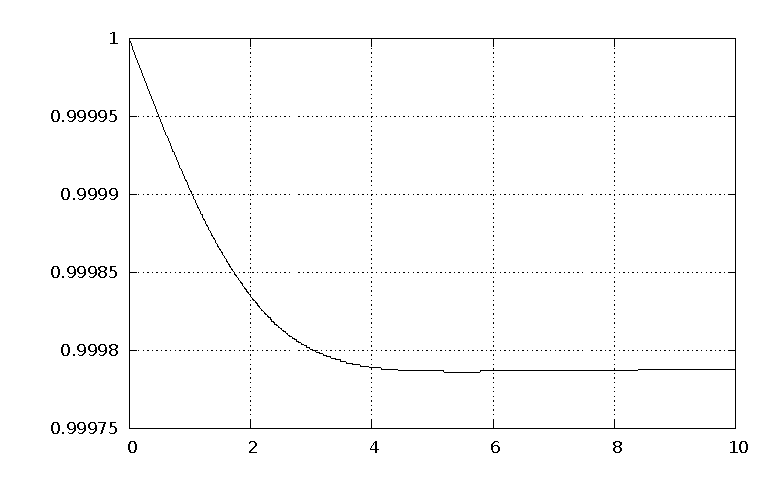
\includegraphics[width=.45\textwidth]
{figures/stokes/ellipse_both_bulk_inner_volume.ps}}
\subfloat[$\gamma\,\mathcal{H}^{1}(\Gamma^m)$]{
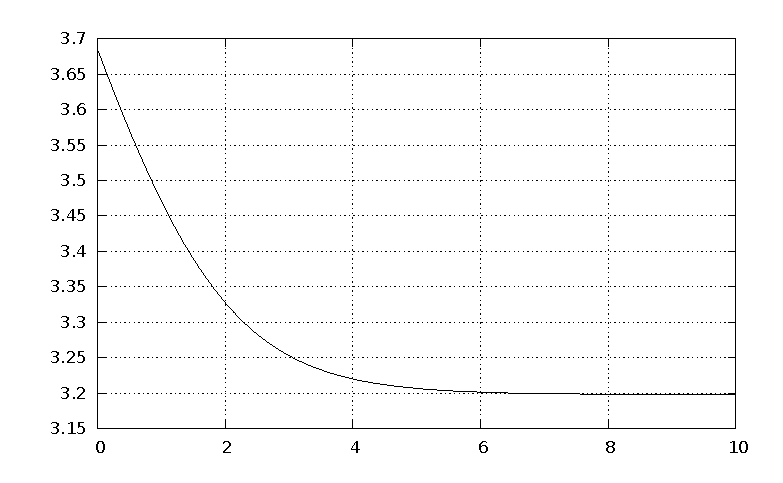
\includegraphics[width=.45\textwidth]
{figures/stokes/ellipse_both_interface_length.ps}}
\caption{Evolutions of the relative inner area and the interface energy for
the simulation in Figure~\ref{fig:ellipse_both}.}
\label{fig:ellipse_both_volumes}
\end{figure}
As a comparison, we show in Figure~\ref{fig:ellipse_smooth} the final snapshot
of the same simulation when no remeshings are performed, i.e. we use $C_r=
\infty$ in (\ref{eq:remesh}). We clearly see that due to the strong deformation
of the interface, this leads to elongated elements in the inner and in the
outer phase of the bulk finite element mesh.
\begin{figure}[htbp]
\centering
\subfloat[$t=10$]{\includegraphics[width=.32\textwidth]
{figures/stokes/ellipse_smooth_1000.ps}}
\caption{($\mu=\gamma=1$) Final pressure solution for a simulation as in
Figure~\ref{fig:ellipse_both}, when no remeshings are performed.}
\label{fig:ellipse_smooth}
\end{figure}

\subsection{Shear flow experiment in 2d}
As the final 2d numerical simulation we present a shear flow experiment. Here
we prescribe the inhomogeneous Dirichlet boundary condition
\begin{equation*}
\vec g(\vec z)=(z_2,0)^T\quad \mbox{on }\partial\Omega\,,
\end{equation*}
and we use the parameters $\mu=1$, $\gamma=3$, $\tau=10^{-2}$ and $T=5$.
The initial interface is discretized with $J_\Gamma = 64$ surface elements,
and the initial bulk mesh has $J_\Omega^0 = 4240$ elements. In
Figure~\ref{fig:shear_2d} we show the evolution of the discrete pressures
for a simulation with $C_r=3$ for the P2--P0 element, while the velocities
are visualized in Figure~\ref{fig:shear_2d_velocity}.
\begin{figure}[htbp]
\centering
\subfloat[$t=0.5$]{
\includegraphics[width=.32\textwidth]{figures/stokes/2d_shear_050.ps}}
\subfloat[$t=1$]{
\includegraphics[width=.32\textwidth]{figures/stokes/2d_shear_100.ps}}
\subfloat[$t=5$]{
\includegraphics[width=.32\textwidth]{figures/stokes/2d_shear_500.ps}}
\caption{($\mu=1,\gamma=3$) Pressure evolution for the 2d shear flow with
$C_r=3$ for the P2--P0 element, uniform mesh.}
\label{fig:shear_2d}
\end{figure}

\begin{figure}[htbp]
\centering
\subfloat[$t=0.5$]{
\includegraphics[width=.32\textwidth]{figures/stokes/2d_shear_velocity_050.ps}}
\subfloat[$t=1$]{
\includegraphics[width=.32\textwidth]{figures/stokes/2d_shear_velocity_100.ps}}
\subfloat[$t=5$]{
\includegraphics[width=.32\textwidth]{figures/stokes/2d_shear_velocity_500.ps}}
\caption{($\mu=1,\gamma=3$) Velocity vector field for the 2d shear flow with
$C_r=3$ for the P2--P0 element, uniform mesh.}
\label{fig:shear_2d_velocity}
\end{figure}

\subsection{Convergence test in 3d} \label{sec:stokes_3d_convergence_results}
Similarly to \S\ref{sec:stokes_2d_convergence_results}, we perform the following
convergence test for a stationary spherical bubble in 3d. Let $\mu = \gamma =
1$. Then the true solution (\ref{eq:radialr},b) reduces to $r(t) =
\frac{1}{2}$, $\vec u(\cdot, t) = \vec 0$ and $p(t) = 4\,\charfcn{\Omega_-(0)}
- \frac{\pi}{12}$ for all $t\geq0$. We approximate this stationary solution on
nearly uniform meshes that feature $J_\Gamma = 32$, $220$ and $596$ interface
elements, and $J_\Omega^0 = 408$, $3590$ and $20473$ bulk elements,
respectively. Here, in contrast to the situation in 2d, we are not able to
define $\Gamma^0$ such that the vertices of $\Gamma^0$ lie on $\Gamma(0)$ and
such that (\ref{eq:constcurv}) is satisfied. As we would like to demonstrate
the ability of our method to recover the discrete stationary solution
(\ref{eq:solsol}) also in 3d, we choose the initial interface $\Gamma^0$ such
that (\ref{eq:constcurv}) holds, at the expense of a nonzero initial error
$\| \Gamma^0 - \Gamma(0) \|_{L^\infty}$, recall (\ref{eq:errorXx}). We obtain
such an initial triangulation with the help of the numerical scheme from
Chapter~\ref{ch:geometric_pdes} for surface diffusion, which is a gradient flow
for surface area that maintains the enclosed volume. See e.g. \cite[Fig.
11]{gflows3d} for an evolution towards a polyhedral approximation of a sphere
that satisfies (\ref{eq:constcurv}), and hence also (\ref{eq:conformal}). We
report on the errors for the P2--P0, P2--P1, P2--$\pdg$
and P2--(P1+P0) elements in Tables~\ref{tab:stokes_stationary_3d_p2p0},
\ref{tab:stokes_stationary_3d_p2p1}, \ref{tab:stokes_stationary_3d_p2p1dg} and
\ref{tab:stokes_stationary_3d_p2p1p0}, respectively. Here we note that, as yet,
for the pairs P2--P0, P2--$\pdg$ and P2--(P1+P0) there exist no proofs in the
literature that the LBB condition (\ref{eq:LBB}) holds, see e.g. the discussion
in \cite[Remark~8.4.3]{BoffiBF13}. However, in practice we encountered no
problems when using these spaces, and our iterative solver always converged to a
solution of the scheme (\ref{eq:HGa}--d). For both sets of simulations we use
the uniform time step size $\tau = 10^{-2}$.
\begin{table*}
\center
\begin{tabular}{rllllr}
\hline
$J_\Gamma$ & $\errorXx$ & $\LerrorUu2$ & $\LerrorPp$ & EOC & CPU[s] \\
\hline
 32 & 2.97986e-02 & 0 & 1.65555e-00 &    - &   385 \\
220 & 5.80971e-03 & 0 & 7.14269e-01 & 1.21 &  4699 \\
596 & 2.42857e-03 & 0 & 3.58466e-01 & 0.99 & 51604 \\
\hline
\end{tabular}
\caption[Stokes 3d P2--P0 stationary bubble errors]
{($\mu=\gamma=1$) Stationary bubble problem on $(-1,1)^3$ over the time
interval $[0,1]$ for the P2--P0 element.}
\label{tab:stokes_stationary_3d_p2p0}
\end{table*}
\begin{table*}
\center
\begin{tabular}{rllllr}
\hline
$J_\Gamma$ & $\errorXx$ & $\LerrorUu2$ & $\LerrorPp$ & EOC & CPU[s] \\
\hline
 32 & 1.56938e-01 & 6.01956e-02 & 2.10996e-00 &    - &   315 \\
220 & 7.28946e-02 & 3.13992e-02 & 1.47595e-00 & 0.52 &  4231 \\
596 & 4.04291e-02 & 1.34276e-02 & 1.09674e-00 & 0.43 & 51287 \\
\hline
\end{tabular}
\caption[Stokes 3d P2--P1 stationary bubble errors]
{($\mu=\gamma=1$) Stationary bubble problem on $(-1,1)^3$ over the time
interval $[0,1]$ for the P2--P1 element.}
\label{tab:stokes_stationary_3d_p2p1}
\end{table*}
\begin{table*}
\center
\begin{tabular}{rllllr}
\hline
$J_\Gamma$ & $\errorXx$ & $\LerrorUu2$ & $\LerrorPp$ & EOC & CPU[s] \\
\hline
 32 & 2.97986e-02 & 0 & 1.65555e-00 &    - &    73 \\
220 & 5.80971e-03 & 0 & 7.14269e-01 & 1.21 &  1018 \\
596 & 2.42857e-03 & 0 & 3.58466e-01 & 0.99 & 17814 \\
\hline
\end{tabular}
\caption[Stokes 3d P2--$\pdg$ stationary bubble errors]
{($\mu=\gamma=1$) Stationary bubble problem on $(-1,1)^3$ over the time
interval $[0,1]$ for the P2--$\pdg$ element.}
\label{tab:stokes_stationary_3d_p2p1dg}
\end{table*}
\begin{table*}
\center
\begin{tabular}{rllllr}
\hline
$J_\Gamma$ & $\errorXx$ & $\LerrorUu2$ & $\LerrorPp$ & EOC & CPU[s] \\
\hline
 32 & 2.97986e-02 & 0 & 1.65749e-00 &    - &    568 \\
220 & 5.80971e-03 & 0 & 7.15353e-01 & 1.21 &   9174 \\
596 & 2.42857e-03 & 0 & 3.59181e-01 & 0.99 & 121110 \\
\hline
\end{tabular}
\caption[Stokes 3d P2--(P1+P0) stationary bubble errors]
{($\mu=\gamma=1$) Stationary bubble problem on $(-1,1)^3$ over the time
interval $[0,1]$ for the P2--(P1+P0) element.}
\label{tab:stokes_stationary_3d_p2p1p0}
\end{table*}

We note that we again recover the discrete stationary solutions
(\ref{eq:solsol}) for the P2--P0, P2--$\pdg$ and P2--(P1+P0) elements while,
as before, the P2--P1 element does not capture exactly the true solution
since this element does not satisfy the hypothesis that $S^m_0 \subset
\pspace^m$ of Theorem~\ref{thm:stat2}. Here this leads to a nonzero error in
the position of the discrete interface, because the vertices of the initial
interface $\Gamma^0$ do not lie on $\Gamma(0)$.

\subsection{Shear flow experiment in 3d}
Finally, we also report on a 3d shear flow experiment.
The initial interface mesh has $J_\Gamma = 596$ elements, while the nearly
uniform bulk mesh is made up of $J_\Omega^0 = 19641$ elements. We prescribe the
inhomogeneous Dirichlet boundary condition
\begin{equation*}
\vec g(\vec z)=(z_3,0,0)^T\quad \mbox{on }\partial\Omega\,,
\end{equation*}
and we use the parameters $\mu=1$, $\gamma=3$, $\tau=10^{-2}$ and $T=5$.
In Figure~\ref{fig:shear_3d} we show the evolution of the discrete interface
for a simulation with $C_r=3$ for the P2--P0 element, while the velocities
are visualized in Figure~\ref{fig:shear_3d_velocity}.
\begin{figure}[htbp]
\centering
\subfloat[$t=0$]{
\includegraphics[width=.32\textwidth]{figures/stokes/3d_shear_000.ps}}
\subfloat[$t=1$]{
\includegraphics[width=.32\textwidth]{figures/stokes/3d_shear_100.ps}}
\subfloat[$t=5$]{
\includegraphics[width=.32\textwidth]{figures/stokes/3d_shear_500.ps}}
\caption{($\mu=1,\gamma=3$) Interface evolution for the 3d shear flow with
$C_r=3$ for the P2--P0 element, uniform mesh.}
\label{fig:shear_3d}
\end{figure}

\begin{figure}[htbp]
\centering
\subfloat[$t=1$]{
\includegraphics[width=.32\textwidth]{figures/stokes/3d_shear_velocity_100.ps}}
\subfloat[$t=5$]{
\includegraphics[width=.32\textwidth]{figures/stokes/3d_shear_velocity_500.ps}}
\caption{($\mu=1,\gamma=3$) Velocity vector field in the plane normal to
$(0,1,0)^T$ and passing through the origin for the 3d shear flow with $C_r=3$
for the P2--P0 element, uniform mesh.}
\label{fig:shear_3d_velocity}
\end{figure}
A plot of the relative inner volume over time is shown in
Figure~\ref{fig:shear_3d_bulk_inner_volume}, where we again observe that our
numerical method maintains the enclosed volume well.

\begin{figure}[htbp]
\centering
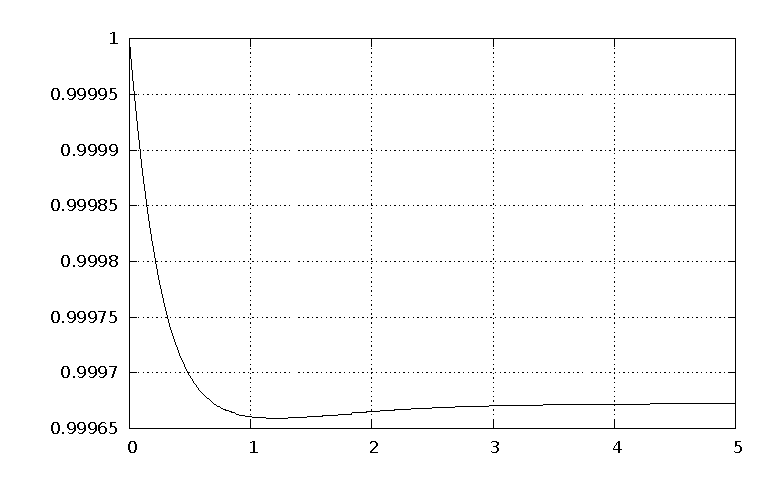
\includegraphics[width=.45\textwidth]
{figures/stokes/3d_shear_bulk_inner_volume.ps}
\caption{A plot of the relative inner volume
$\frac{\mathcal{L}^3(\Omega^m_-)}{\mathcal{L}^3(\Omega^0_-)}$
over time for the simulation in Figure~\ref{fig:shear_3d}.}
\label{fig:shear_3d_bulk_inner_volume}
\end{figure}
